\documentclass[tikz, border=5mm]{standalone}
\usepackage{tikz}
% \usetikzlibrary {arrows.meta}
% \usetikzlibrary{positioning,arrows.meta, calc, quotes, angles}
\usetikzlibrary{positioning,arrows.meta, calc, quotes, angles, decorations.pathmorphing, patterns}

\usepackage{tikz-3dplot}
\usepackage{sansmath}     % Für serifenlose Schrift in Formeln

\usepackage{eurosym}  % euro symbol € 
\usepackage{amsmath,amssymb,latexsym,amsfonts,bbm, bm, bbold}
\usepackage{mathtools}
\usepackage[b]{esvect} % For \vv (option [d] is a nice default)

\usepackage{pgfplots}
\pgfplotsset{compat=1.18}
\usepackage{siunitx}
\DeclareSIUnit{\litre}{l}
\DeclareSIUnit{\calorie}{cal}
\DeclareSIUnit{\barPr}{bar}
\sisetup{
    locale = DE, 
    angle-symbol-degree = ^\circ,
    separate-uncertainty, 
    inter-unit-product = {},
    range-units = brackets, 
    list-units = single, 
    per-mode=symbol-or-fraction,
    range-phrase = { bis }
}

\newcommand{\ehat}[1]{\hat{\bm{e}}_{#1}}
\newcommand{\dd}{\mathrm{d}}
\newcommand{\ivec}[1]{\vv{#1}} % using esvect package
\newcommand{\ivecS}[2]{\vv*{#1}{\!#2}} % using esvect package

\begin{document}


%%%   -----------------------------------------------------------
%%%   -----------------------------------------------------------
%%%   -----------------------------------------------------------


% Eine schiefe Ebene mit einem Winkel alpha (eingezeichnet) gegen die Horizontale in leichtem rot 
% Ein Kreis (Rad) mit Radius r rollt ohne zu rutschen die Ebene hinunter. Der Schwerpunkt des Rades ist markiert.
% Die Kräfte Gewicht F_G und F_N (Normalkraft) sind eingezeichnet.

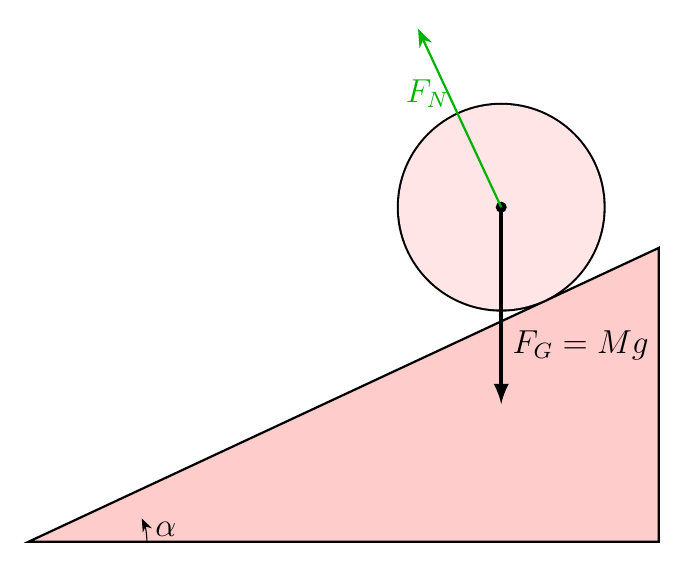
\begin{tikzpicture}[
    scale=1.0,
    >=Stealth,
    font=\small\sffamily
]

    % --- Definitionen ---
    \def\R{1.3} % Radius des Rades
    \def\alphaV{25} % Winkel der schiefen Ebene
    \def\lenEbene{8} % Länge der schiefen Ebene

    % --- Schiefe Ebene zeichnen ---
    \fill[red!20] (0,0) -- (\lenEbene,0) -- (\lenEbene, {\lenEbene*tan(\alphaV)}) -- (0,0) -- cycle;
    \draw[thick] (0,0) -- (\lenEbene,0) -- (\lenEbene, {\lenEbene*tan(\alphaV)}) -- cycle;
    % --- Rad zeichnen ---
    \coordinate (Center) at (6, {6*tan(\alphaV) + \R + 0.15}); % Mittelpunkt des Rades
    \draw[line width=1.5pt] (Center) circle (\R); % Rad
    \fill[red!10] (Center) circle (\R); % rote Füllung
    \fill[black] (Center) circle (2pt); % Schwerpunkt

    % --- Kräfte zeichnen ---
    % Gewichtskraft F_G
    \draw[-{latex}, black, line width=1.5pt] (Center) -- ++(0,-2.5) node[midway, pos=0.7, right] {\large $F_G = M \ivec{g}$};

    % Normalkraft F_N
    \draw[->, green!70!black, thick] (Center) -- ++({\alphaV+90}:2.5) node[midway, above left] {\large $F_N$};

    % --- Winkel alpha beschriften ---
    \draw[->] (1.5,0) arc(0:\alphaV:0.7) node[midway, right] {\large $\alpha$};
\end{tikzpicture}






%%%   -----------------------------------------------------------
%%%   -----------------------------------------------------------
%%%   -----------------------------------------------------------


% % Ein dreidimensionales Koordinatensystem mit den Achsen x, y und z
% % Ein Punkt P im Raum mit den Koordinaten (x, y, z) und ein Pfeil der vom Ursprung zu diesem Punkt zeigt
% % Ein Vektor F der am Punkt P endet und in eine bestimmte Richtung zeigt
% % F wird in seine Komponenten F_n, F_t und F_b zerlegt, die jeweils normal, tangential und binormal zum Vektor r sind
% % Ein grüner Quader ist der Körper, der den Punkt P enthält
% \begin{tikzpicture}[
%     scale=1.0,
%     >=Stealth,
%     font=\small\sffamily
% ]

%     % --- Koordinaten-Definition ---
%     \coordinate (Origin) at (0,0,0);
%     \coordinate (XEnd) at (5,0,0);
%     \coordinate (YEnd) at (0,5,0);
%     \coordinate (ZEnd) at (0,0,5);

%     % Punkt P im Raum
%     \coordinate (P) at (3,2,4);

%     % Vektor F am Punkt P
%     \coordinate (FEnd) at (4,4,5);

%     % --- Achsen zeichnen ---
%     \draw[->, thick] (Origin) -- (XEnd) node[below right] {\large $x$};
%     \draw[->, thick] (Origin) -- (YEnd) node[above left] {\large $y$};
%     \draw[->, thick] (Origin) -- (ZEnd) node[above right] {\large $z$};

%     % --- Punkt P und Pfeil zum Ursprung ---
%     \fill[black] (P) circle (2pt);
%     \draw[->, blue, thick] (Origin) -- (P) node[midway, below right] {\large $\vec{r}$};
%     \node[above right] at (P) {\large $P(x,y,z)$};

%     % --- Grüner Quader um Punkt P ---
%     \draw[fill=green!20, opacity=0.5] (2.5,1.5,3.5) -- (3.5,1.5,3.5) -- (3.5,2.5,3.5) -- (2.5,2.5,3.5) -- cycle; % Boden
%     \draw[fill=green!20, opacity=0.5] (2.5,1.5,4.5) -- (3.5,1.5,4.5) -- (3.5,2.5,4.5) -- (2.5,2.5,4.5) -- cycle; % Decke
%     \draw[fill=green!20, opacity=0.5] (2.5,1.5,3.5) -- (2.5,2.5,3.5) -- (2.5,2.5,4.5) -- (2.5,1.5,4.5) -- cycle; % Seite 1
%     \draw[fill=green!20, opacity=0.5] (3.5,1.5,3.5) -- (3.5,2.5,3.5) -- (3.5,2.5,4.5) -- (3.5,1.5,4.5) -- cycle; % Seite 2
%     \draw[fill=green!20, opacity=0.5] (2.5,1.5,3.5) -- (3.5,1.5,3.5) -- (3.5,1.5,4.5) -- (2.5,1.5,4.5) -- cycle; % Seite 3
%     \draw[fill=green!20, opacity=0.5] (2.5,2.5,3.5) -- (3.5,2.5,3.5) -- (3.5,2.5,4.5) -- (2.5,2.5,4.5) -- cycle; % Seite 4

%     % --- Vektor F am Punkt P ---
%     \draw[->, red, thick] (P) -- (FEnd) node[midway, above right] {\large $\vec{F}$};

%     % --- Komponenten von F ---
%     % Normal-Komponente F_n
%     % \draw[dashed, green!70!black] (P) -- ($(P)!1!(FEnd)$ |- $(P)$);
%     % \draw[->, green!70!black, thick] ($(P)$) -- ($(P)!1!(FEnd)$ |- $(P)$) node[midway, left] {\large $\vec{F}_n$};

%     % % Tangential-Komponente F_t
%     % \draw[dashed, orange!70!black] ($(P)!1!(FEnd)$ |- $(P)$) -- ($(FEnd)$);
%     % \draw[->, orange!70!black, thick] ($(P)!1!(FEnd)$ |- $(P)$) -- ($(FEnd)$) node[midway, above] {\large $\vec{F}_t$};

%     % Binormal-Komponente F_b
%     \draw[dashed, purple!70!black] (P) -- ($(FEnd)$);
%     \draw[->, purple!70!black, thick] (P) -- ($(FEnd)$) node[midway, right] {\large $\vec{F}_b$};
% \end{tikzpicture}




%%%   -----------------------------------------------------------
%%%   -----------------------------------------------------------
%%%   -----------------------------------------------------------


% Ein Flächenelement in Polarkoordinaten mit Beschriftungen für r, dphi, dr und dA = r dphi dr
% Ein strichlierter Kreis im Hintergrund um den Kreis zu andeuten
% Das Flächenelement soll orange gefärbt sein
% \begin{tikzpicture}[>=Stealth, scale=1.2]
%         % Definitionen
%         \def\R{3.5}
%         \def\angA{30}
%         \def\angB{60}
%         \def\rIn{2.0}
%         \def\rOut{2.9}
%         \definecolor{boxcolOrange}{RGB}{255, 191, 77} % or use your preferred RGB values
%         \definecolor{boxcolDarkOrange}{RGB}{255, 140, 0}

%         % Koordinatensystem
%         \draw[->, line width=1pt] (-0.5,0) -- (4,0) node[right] {$x$};
%         \draw[->, line width=1pt] (0,-0.5) -- (0,4) node[above] {$y$};
        
%         % Kreisbogen andeuten (gestrichelt)
%         \draw[dashed, gray] (0,0) circle (\rOut);
        
%         % Segment zeichnen (Flächenelement)
%         \fill[fill=boxcolOrange] (\angA:\rIn) arc(\angA:\angB:\rIn) -- (\angB:\rOut) arc(\angB:\angA:\rOut) -- cycle;
%         \draw[thick, fill=boxcolOrange] (\angA:\rIn) arc(\angA:\angB:\rIn) -- (\angB:\rOut) arc(\angB:\angA:\rOut) -- cycle;
        
%         % Linien vom Ursprung
%         \draw[thin] (0,0) -- (\angA:\rOut);
%         \draw[thin] (0,0) -- (\angB:\rOut);
        
%         % Beschriftungen
%         % dr
%         \draw[|<->|] (\angA-5:\rIn) -- (\angA-5:\rOut) node[midway,pos=0.6, below] {$\dd r$};
        
%         % r dphi (Bogenlänge)
%         \draw[<->] (\angA:\rIn+0.4) arc(\angA:\angB:\rIn+0.4) node[midway, above, rotate=-42] {$r \cdot \dd \varphi$};
        
%         % r Vektor
%         \draw[->, blue, line width=1.2pt] (0,0) -- (\angA:{\rIn+0.4}) node[midway, below right] {$r$};
        
%         % Winkel dphi
%         \draw[<->] (\angA:1.) arc(\angA:\angB:1.) node[midway, above right] {$\dd \varphi$};
        
%         % dA Label
%         \node[boxcolDarkOrange] at (45:4.2) {$\dd A = r \, \dd \varphi \, \dd r$};
%         \draw[-, black, line width=0.5pt] (55:\rOut) -- (55:3.5);
% \end{tikzpicture}



%%%   -----------------------------------------------------------
%%%   -----------------------------------------------------------
%%%   -----------------------------------------------------------

% Ein (x,y) Koordinatensystem mit Pfeilen die die x- und y-Achse darstellen
% Ein Dreieck mit den Eckpunkten (0,0), (a,0) und (0,b)
% Die Fläche des Dreiecks soll schraffiert dargestellt werden
% Die Ticks sollen bei x=0, x=a und y=0, y=b sein

% \begin{tikzpicture}[
%         scale=1.2,
%         >=latex, 
%         font=\small\sffamily
%     ]

%     % --- Koordinaten-Definition ---
%     \def\a{6} % Länge der Basis des Dreiecks
%     \def\b{4} % Höhe des Dreiecks
%     \def\k{0.6} % Steigung der Hypotenuse ((b-1)/(a-1))

%     % Achsen-Endpunkte
%     \coordinate (Origin) at (0,0);
%     \coordinate (A) at (1,1);
%     \coordinate (XEnd) at (\a+1,0);
%     \coordinate (YEnd) at (0,\b+1);

%     % --- Fläche füllen ---
%     \fill[red!20] 
%         (A) -- (\a,1) -- (1,\b) -- cycle;

%     % --- Achsen zeichnen ---
%     \draw[->, thick] (-0.5,0) -- (XEnd) node[below] {\Large $x$};
%     \draw[->, thick] (0,-0.5) -- (YEnd) node[left] {\Large $y$};

%     % --- Ticks und Labels X-Achse ---
%     \draw[thick] (\a, -0.15) -- (\a, 0.15) node[below=0.3cm] {\large $a$};
%     \draw[thick] (1, -0.15) -- (1, 0.15) node[below=0.3cm] {\large $0$};
%     \draw[thick] (2, -0.1) -- (2, 0.1) node[below=0.3cm] {\large $x_1$};
%     \draw[thick] (4, -0.1) -- (4, 0.1) node[below=0.3cm] {\large $x_2$};
%     \draw[thick] (-0.1, \b-\k*1) -- (0.1, \b-\k*1) node[left=0.3cm] {\large $y_1$};
%     \draw[thick] (-0.1, \b-\k*3) -- (0.1, \b-\k*3) node[left=0.3cm] {\large $y_2$};

%     % --- Ticks und Labels Y-Achse ---
%     \draw[thick] (-0.15, \b) -- (0.15, \b) node[left=0.3cm] {\large $b$};
%     \draw[thick] (-0.15, 1) -- (0.15, 1) node[left=0.3cm] {\large $0$};

%     % --- Das Dreieck als Linie zeichnen ---
%     \draw[thick] (1,1) -- (\a,1) -- (1,\b) -- cycle;

%     % --- blaue Linie von (2,1) nach (2, \b-\k*1) ---
%     \draw[line width=2pt, blue] (2,1) -- (2,\b-\k*1) node[midway,pos=0.4, right] {\large $g(x_1)$};
%     \draw[line width=2pt, blue] (4,1) -- (4,\b-\k*3) node[midway,pos=0.4, right] {\large $g(x_2)$};

%     % --- strichlierte Linie von (0,g(x1)) nach (2,g(x1)) ---
%     \draw[dashed, thin] (0,\b-\k*1) -- (2,\b-\k*1);
%     \draw[dashed, thin] (0,\b-\k*3) -- (4,\b-\k*3);

% \end{tikzpicture}



%%%   -----------------------------------------------------------
%%%   -----------------------------------------------------------
%%%   -----------------------------------------------------------

% p-V-Diagramm einer isothermen Expansion mit Beschriftungen um die Arbeit zu verdeutlichen
% die Arbeit W ist das Integral unter der Kurve im p-V-Diagramm
% \begin{tikzpicture}[
%         scale=1.1,
%         >=latex, 
%         font=\small
%         ]
%         % Rasterhilfslinien (optional, leicht angedeutet)
%         \draw[step=1cm, gray!20, very thin] (0,0) grid (7.8, 4.8);

%         % --- DECLARE FUNCTION ---
%         % Wir definieren die Isotherme p(x) = k / x
%         % Skalierung: Um visuell dem Bild zu entsprechen. 
%         \tikzset{declare function={
%             isotherm(\v) = 10 / \v;
%         }}

%         % Definition der Punkte V1 und V2
%         \def\Va{3.0} % Startvolumen
%         \def\Vb{5.5} % Endvolumen

%         % 2. Fläche schraffieren/füllen (Das Integral)
%         % Wir füllen den Bereich unter der Kurve zwischen Va und Vb
%         \fill[violet!20] (\Va,0) -- (\Va, {isotherm(\Va)}) 
%             plot[domain=\Va:\Vb, samples=50] (\x, {isotherm(\x)}) 
%             -- (\Vb, 0) -- (\Va,0) -- cycle;

%         % Label für die Arbeit -W
%         \node[violet!60!black] at (4.1, 1.0) {\Large $-W$};

%         % 3. Die Kurve zeichnen (Isotherme)
%         \draw[red, thick, domain=2.1:7.5, samples=100] plot (\x, {isotherm(\x)});

%         % 4. Punkte und Labels einzeichnen
        
%         % Punkt 1 (Start)
%         \coordinate (P1) at (\Va, {isotherm(\Va)});
%         \fill[black] (P1) circle (2pt);
        
%         % Label Box für Punkt 1
%         \node[draw, fill=white, align=center, anchor=south west] (L1) at (3.0, 3.5) {\large $p_1, V_1, T$};
%         \draw[thin] (L1.south west) -- (P1);

%         % Punkt 2 (Ende)
%         \coordinate (P2) at (\Vb, {isotherm(\Vb)});
%         \fill[black] (P2) circle (2pt);

%         % Label Box für Punkt 2
%         \node[draw, fill=white, align=center, anchor=south west] (L2) at (5.5, 2.0) {\large $p_2 < p_1, V_2 > V_1, T$};
%         \draw[thin] (L2.south west) -- (P2);

%         % 1. Definition der Funktion (Hyperbelast)
%         % p(V) = const / V. Hier wählen wir k = 2.5 für die Optik
%         \draw[->, line width=1.2pt] (0,0) -- (8,0) node[below,right] {\Large $V$};
%         \draw[->, line width=1.2pt] (0,0) -- (0,5) node[above left] {\Large $p$};

% \end{tikzpicture}








%%%   -----------------------------------------------------------
%%%   -----------------------------------------------------------
%%%   -----------------------------------------------------------




% p-V-Diagramm des Carnot-Kreisprozesses mit Beschriftungen
% \begin{tikzpicture}[
%         scale=1.2,
%         >={Stealth}, % Pfeilspitzen-Stil
%         font=\small\sffamily
%     ]

%     % --- Koordinaten-Definition ---
%     % Diese Punkte definieren die Ecken des Zyklus (V, p)
%     % 1: Hochdruck/Kleines Volumen
%     \coordinate (P1) at (1.2, 5.0); 
%     % 2: Isotherme Expansion von 1
%     \coordinate (P2) at (4.0, 3.2); 
%     % 3: Adiabatische Expansion von 2
%     \coordinate (P3) at (5.5, 1.4); 
%     % 4: Isotherme Kompression von 3
%     \coordinate (P4) at (2.2, 2.2); 

%     % Achsen-Endpunkte
%     \coordinate (Origin) at (0,0);
%     \coordinate (XEnd) at (6.5,0);
%     \coordinate (YEnd) at (0,6.0);

%     % --- Fläche füllen ---
%     % Wir füllen zuerst, damit Gitterlinien/Achsen darüber liegen können, 
%     % falls gewünscht. Hier füllen wir den Zyklus rot/orange.
%     \fill[fill=red!25] 
%         (P1) to[out=-25, in=160] (P2) % Isotherme T1
%              to[out=-70, in=115] (P3) % Adiabate
%              to[out=165, in=-15] (P4) % Isotherme T2
%              to[out=110, in=-75] (P1) % Adiabate
%              -- cycle;

%     % --- Hilfslinien zu den Achsen (V1...V4) ---
%     \draw[dashed, thin] (P1) -- (P1 |- Origin) node[below] {\large $V_1$};
%     \draw[dashed, thin] (P2) -- (P2 |- Origin) node[below] {\large $V_2$};
%     \draw[dashed, thin] (P3) -- (P3 |- Origin) node[below] {\large $V_3$};
%     \draw[dashed, thin] (P4) -- (P4 |- Origin) node[below] {\large $V_4$};

%     % --- Achsen zeichnen ---
%     \draw[->, thick] (-0.5,0) -- (XEnd) node[below] {\large $V$};
%     \draw[->, thick] (0,-0.5) -- (YEnd) node[left] {\large $p$};

%     % --- Den Zyklus zeichnen (Umrandung) ---
%     \draw[thick] (P1) to[out=-25, in=160] node[midway, above right=2pt] {\large $T_1$} (P2);
%     \draw[thick] (P2) to[out=-70, in=115] (P3);
%     \draw[thick] (P3) to[out=165, in=-15] node[midway, below left=2pt] {\large $T_2$} (P4);
%     \draw[thick] (P4) to[out=110, in=-75] (P1);

%     % --- Eckpunkte beschriften (1, 2, 3, 4) ---
%     \node[above left] at (P1) {\large 1};
%     \node[above right] at (P2) {\large 2};
%     \node[right] at (P3) {\large 3};
%     \node[below left] at (P4) {\large 4};

%     % --- Wärmemengen-Pfeile (Q1, Q2) ---
%     % Q1 (Wärmezufuhr, rot) - von oben in die Fläche
%     \draw[->, ultra thick, red!80!black] (2.8, 4.5) -- (2.8, 3.3) node[midway, right] {\large $\Delta Q_1$};
    
%     % Q2 (Wärmeabfuhr, schwarz) - von der Fläche nach unten
%     \draw[->, ultra thick, black] (3.8, 2.3) -- (3.8, 1.1) node[midway, right] {\large $\Delta Q_2$};

%     % --- Beschriftungen für Kurventypen (Isotherme, Adiabate) ---
%     % Isotherme (zeigt auf obere Kurve)
%     \node (iso_label) at (5.0, 4.8) {\large Isotherme};
%     \draw[thin] (iso_label.south west) -- (3.2, 4.0);

%     % Adiabate (zeigt auf rechte Kurve)
%     \node (adia_label) at (6.0, 3.0) {\large Adiabate};
%     \draw[thin] (adia_label.west) -- (4.8, 2.2);

% \end{tikzpicture}


%     \caption{Das $p$-$V$-Diagramm des Carnot-Kreisprozesses. Der Prozess wird von zwei Isothermen (Temperatur $T_1$ und $T_2$) und zwei Adiabaten begrenzt. Die eingeschlossene Fläche entspricht der verrichteten Arbeit.}
%     \label{fig: carnot_prozess_pv}
% \end{figure}



%%%   -----------------------------------------------------------
%%%   -----------------------------------------------------------
%%%   -----------------------------------------------------------





% % Zeit-Temperatur Diagramm für Wasser von -20°C Eis bis hin zu Dampf bei 120°C
% % Der Zeitverlauf ist in rot dargestellt, mit Beschriftungen für die Phasenübergänge und 
% % Aggregatzustände und Pfeilen für die latente Wärme und die Erwärmungsraten
% \begin{tikzpicture}[
%     scale=1.0, font=\small,
%     axis/.style={-{Stealth}, line width=1.0pt},
%     box/.style={draw, fill=blue!10, rounded corners=2pt, minimum height=0.6cm, align=center, font=\footnotesize},
%     curve/.style={line width=1.5pt, red!80!black},
%     guide/.style={dashed, thin, gray}
% ]

%     % --- Definition der Koordinaten (Zeit t und Temperatur T) ---
%     % Y-Achse
%     \def\yStart{0.5}   % Start bei z.B. -20 Grad
%     \def\yMelt{2.0}    % 0 Grad
%     \def\yBoil{5.5}    % 100 Grad
%     \def\yEnd{7.0}     % > 100 Grad

%     % X-Achse (Zeitpunkte)
%     \def\xZero{0}
%     \def\xOne{1.0}     % Ende Eis-Erwärmung
%     \def\xTwo{2.0}     % Ende Schmelzen
%     \def\xThree{5.0}   % Ende Wasser-Erwärmung
%     \def\xFour{10.0}   % Ende Verdampfen (Langes Plateau!)
%     \def\xEnd{10.6}    % Ende Dampf-Erwärmung

%     % Y-Position der Beschriftungsboxen oben
%     \def\yBox{6.3}

%     % --- 1. Achsen zeichnen ---
%     \draw[axis] (0, \yMelt) -- (\xEnd+0.5, \yMelt) node[right] {$t \,[\si{\second}]$}; 
%     \draw[axis] (0, 0) -- (0, \yBox+1) node[left] {\large $T\, [\si{\celsius}]$};
    
%     % --- 2. Ticks und Labels Y-Achse ---
%     \draw[thick] (-0.15, \yStart) -- (0.15, \yStart) node[left=0.3cm] {$T_a$}; % Anfang
%     \draw[thick] (-0.15, \yMelt) -- (0.15, \yMelt) node[left=0.3cm] {$T_s = \SI{0}{\celsius}$};
%     \draw[thick] (-0.15, \yBoil) -- (0.15, \yBoil) node[left=0.3cm] {$T_v = \SI{100}{\celsius}$};
%     \draw[thick, dashed, gray] (0, \yBoil) -- (\xEnd+0.5, \yBoil); % Hilfslinie bei Siedetemp.
%     % --- 3. Kurve zeichnen ---
%     \draw[curve] 
%         (\xZero, \yStart) coordinate (Start)
%         -- (\xOne, \yMelt) coordinate (MeltStart)
%         -- (\xTwo, \yMelt) coordinate (MeltEnd)
%         -- (\xThree, \yBoil) coordinate (BoilStart)
%         -- (\xFour, \yBoil) coordinate (BoilEnd)
%         -- (\xEnd, \yEnd) coordinate (End);

%     % --- 4. Hilfslinien & Ticks X-Achse ---
%     % t1
%     \draw[guide] (MeltStart) -- (\xOne, 0) node[below, black] {$t_1$};
%     % t2
%     \draw[guide] (MeltEnd) -- (\xTwo, 0) node[below, black] {$t_2$};
%     % t3
%     \draw[guide] (BoilStart) -- (\xThree, 0) node[below, black] {$t_3$};
%     % t4
%     \draw[guide] (BoilEnd) -- (\xFour, 0) node[below, black] {$t_4$};

%     % --- 5. Beschriftungsboxen (Phasen) ---
%     % Schmelzen
%     \node[align=center, text width=1.8cm] at ({(\xOne+\xTwo)/2}, \yMelt+0.5) {Schmelzen};
%     % Verdampfen
%     \node[align=center, text width=3.8cm] at ({(\xThree+\xFour)/2}, \yBoil+0.5) {Verdampfen};
    
%     % --- 6. Zusätzliche Infos im Plot ---
%     % Aggregatzustände unter die Kurve schreiben
%     \node[red!60!black, font=\footnotesize] at ({(\xZero+\xOne)/2}, \yStart+0.1) {fest};
%     \node[red!60!black, font=\footnotesize] at ({(\xTwo+\xThree)/2}, \yMelt+0.9) {flüssig};
%     \node[red!60!black, font=\footnotesize] at (\xFour+0.86, \yEnd-1.2) {gasförmig};

%     % Pfeil für Latente Wärme
%     \draw[<->, >=Latex, thin] (\xThree, \yBoil-0.3) -- (\xFour, \yBoil-0.3) node[midway, below] {$\Delta Q = m \cdot \lambda_v$};

%     % dT/dt Pfeile während der Erwärmungsphasen
%     \draw[->, >=Latex, thin] ({(\xZero+\xOne)/2}, \yStart+0.65) -- (\xTwo+0.35, \yStart+0.1) node[right] {$\frac{\dd T}{\dd t} \propto \frac{1}{C_V\text{(fest)}}$};
%     \draw[->, >=Latex, thin] ({(\xTwo+\xThree)/2 + 0.1}, \yMelt+1.77) -- (\xThree+0.35, \yMelt+1) node[right] {$\frac{\dd T}{\dd t} \propto \frac{1}{C_V\text{(flüssig)}}$};
%     \draw[->, >=Latex, thin] (\xFour+0.3, \yBoil+1) -- (\xFour-0.35, \yBoil+1.5) node[left] {$\frac{\dd T}{\dd t} \propto \frac{1}{C_V\text{(gas)}}$};

% \end{tikzpicture}
   

%%%   -----------------------------------------------------------
%%%   -----------------------------------------------------------
%%%   -----------------------------------------------------------




% % Zeit-Temperatur Diagramm für das Erhitzen und Sieden von Wasser (20 auf 100 Grad)
% % --- mit Beschriftungsboxen für Erwärmen und Sieden/Verdampfen ---
% \begin{tikzpicture}[
%     axis/.style={-{Stealth}, line width=1.2pt},
%     box/.style={draw, fill=blue!15, minimum height=0.8cm, align=center}
% ]

% \def\xTzero{0.3}      % Startzeit 0 s
% \def\xTone{2.5}    % Zeitpunkt t1 (skaliert)
% \def\xTtwo{10}      % Zeitpunkt t2 (skaliert)

% \def\yInitial{1.5}  % Starttemperatur 20 °C
% \def\yBoil{5.5}     % Siedetemperatur 100 °C
% \def\yBoxCenter{6.5} % y-Position der Boxen

% % Achsen zeichnen
% \draw[axis,line width=1.8pt] (-0.5, 0) -- (12, 0) node[right] {\Large $t \,[\si{\second}]$};
% \draw[axis,line width=1.8pt] (0, -0.5) -- (0, 7) node[above] {\Large $T\, [\si{\celsius}]$};

% % Ticks auf den Achsen
% \draw[line width=1pt] (\xTzero, -0.15) -- (\xTzero, 0.15); % Tick bei 0
% \draw[line width=1pt] (\xTone, -0.15) -- (\xTone, 0.15); % Tick bei 0
% \draw[line width=1pt] (\xTtwo, -0.15) -- (\xTtwo, 0.15); % Tick bei 0
% \draw[line width=1pt] (-0.15, \yInitial) -- (0.15, \yInitial);
% \draw[line width=1pt] (-0.15, \yBoil) -- (0.15, \yBoil);

% % Achsenbeschriftungen
% \node[left] at (-0.15, \yInitial) {\large $\SI{20}{\celsius}$};
% \node[left] at (-0.15, \yBoil) {\large $\SI{100}{\celsius}$};
% \node[below] at (\xTzero, -0.15) {\large $0$};
% \node[below] at (\xTone, -0.15) {\large $t_1$};
% \node[below] at (\xTtwo, -0.15) {\large $t_2$};

% % Temperaturverlauf
% \draw[line width=1.4pt, black] (\xTzero, \yInitial) -- (\xTone, \yBoil) -- (\xTtwo, \yBoil);
% % Gestrichelte Hilfslinien
% \draw[dotted] (\xTone, 0) -- (\xTone, \yBoil);
% \draw[dotted] (\xTtwo, 0) -- (\xTtwo, \yBoil);
% % Markierungspunkt am Ende
% \filldraw[black] (\xTtwo, \yBoil) circle (2.5pt);

% % Anmerkung mit Pfeil
% \draw[-{Stealth},, thick] (\xTtwo-1, \yBoil-1.1) -- (\xTtwo-0.1, \yBoil-0.1);
% \node[above left, align=left] at (\xTtwo-1, \yBoil-1.6) {Wasser komplett verdampft};

% % Boxen für die Phasen
% % Berechnung der Breiten und Positionen
% \pgfmathsetmacro{\widthPhaseOne}{\xTone - \xTzero}
% \pgfmathsetmacro{\widthPhaseTwo}{\xTtwo - \xTone}
% \pgfmathsetmacro{\centerPhaseOne}{(\xTone + \xTzero) / 2}
% \pgfmathsetmacro{\centerPhaseTwo}{(\xTtwo + \xTone) / 2}

% \node[box, text width=\widthPhaseOne cm-0.2cm] at (\centerPhaseOne, \yBoxCenter) {Erwärmen};
% \node[box, text width=\widthPhaseTwo cm-0.2cm] at (\centerPhaseTwo, \yBoxCenter) {Sieden / Verdampfen};

% \end{tikzpicture}


%%%   -----------------------------------------------------------
%%%   -----------------------------------------------------------
%%%   -----------------------------------------------------------



% Eine Darstellung der Maxwell-Boltzmann Verteilung als Produkt von Parabel v^2 (blau strichliert) und Exponentialfunktion e^(-v^2) (grün strichliert) und dem Ergebnis (rot durchgezogen)
% \begin{tikzpicture}[xscale=1.2, yscale=4.5, >=Latex, font=\small]
%         % Achsen
%         \draw[->] (0,0) -- (4,0) node[right] {$v$};
%         \draw[->] (0,0) -- (0,1.1) node[above] {Wahrscheinlichkeit};
        
%         % 1. Parabel (v^2) - Skaliert für die Optik
%         \draw[blue, thick, dashed, domain=0:2.1] plot (\x, {0.2*\x*\x}) node[right] {$v^2$ (Volumen)};
        
%         % 2. Exponential (e^-v^2)
%         \draw[green!60!black, thick, dashed, domain=0:3.7] plot (\x, {exp(-0.8*\x*\x)}) node[below=1pt, xshift=-1cm] {$e^{-v^2}$ (Boltzmann)};
        
%         % 3. Produkt (Maxwell-Boltzmann)
%         \draw[red, ultra thick, domain=0:3.7, samples=100] plot (\x, {2.0 * \x^2 * exp(-0.8*\x*\x)}) node[above=4pt] {Resultat $f(v)$};
        
%         % Beschriftung
%         \node[below left] at (0,0) {0};
% \end{tikzpicture}



%%%   -----------------------------------------------------------
%%%   -----------------------------------------------------------
%%%   -----------------------------------------------------------


% Eine Gegenüberstellung von zwei Zylindern: Links ein Gas mit exponentiell abnehmendem Druck und Dichte, rechts eine Flüssigkeit mit konstantem Druck und Dichte
% \begin{tikzpicture}[>=Latex]
%     % =========================
%     % Gemeinsame Parameter
%     % =========================
%     \def\cylW{4.4}       % Breite des Zylinders
%     \def\cylH{5.0}       % Gesamthöhe
%     \def\hBase{1.2}      % Referenzhöhe h (etwas angehoben, damit man sie sieht)
%     \def\dh{1.0}         % Abstand dh
%     \def\offset{8.0}     % Abstand zwischen den Zylindern
%     \def\AOffset{0.5}    % Vertikaler Versatz für die A-Beschriftung
%     % ============================================================
%     % LINKER ZYLINDER: GAS (Kompressibel)
%     % ============================================================
%     \begin{scope}
%         \node[above, font=\bfseries] at (\cylW/2, \cylH+0.5) {Gas (kompressibel)};

%         % 1. Füllung: Linearer Farbverlauf (orange -> weiß)
%         % Visualisiert abnehmende Dichte mit der Höhe
%         \shade[bottom color=orange!60, top color=white] (0,0) rectangle (\cylW, \cylH*0.99);

%         % 2. Zylinderwände
%         \draw[thick] (0,0) -- (0,\cylH);
%         \draw[thick] (\cylW,0) -- (\cylW,\cylH);
%         \draw[thick] (0,0) -- (\cylW,0); % Boden

%         % 3. Markierungslinien für das Volumenelement
%         % Untere Linie bei h
%         \draw[line width=4pt, orange!80!black, opacity=0.7] (0, \hBase) -- (\cylW, \hBase);

%         % 4. Koordinatenachse z
%         \draw[->, ultra thick] (-1.4, \cylH*0.7) -- (-1.4, \cylH) node[right, above] {\Large $z$};
        
%         % 5. Druck-Pfeil und Formel
%         % Exponentielle Abnahme
%         \draw[->, ultra thick, orange!90!black] (\cylW/2, \cylH-1.2) -- (\cylW/2, \hBase+0.1) 
%             node[pos=-0.2, align=center, fill=white, fill opacity=0.0, text opacity=1, rounded corners] 
%             {$p(z) = p_0 \cdot e^{-\frac{z}{H}}$\\[0.3em] \small (Exponentielle Abnahme)};

%         % 6. Beschriftungen
%         % Links (Höhen)
%         \node[left=0.2] at (0, \hBase) {\large $p(h), \rho(h)$};
%         \draw[line width=2pt] (-0.2, \hBase) -- (0.0, \hBase); % Tick mark
%         % p_0
%         \node[left=0.2] at (0, 0) {\large $p_0, \rho_0$};
%         \draw[line width=2pt] (-0.2, 0.03) -- (0.0, 0.03); % Tick mark

%         % Rechts (Dichte/Druck Werte)
%         % Dichte variiert mit der Höhe

%         % Mitte (Fläche A)
%         \node[orange!90!black, font=\bfseries] at (\cylW/2, \hBase - \AOffset) {\Large $A$};
%     \end{scope}

%     % ============================================================
%     % RECHTER ZYLINDER: FLÜSSIGKEIT (Inkompressibel)
%     % ============================================================
%     \begin{scope}[xshift=\offset cm]
%          \node[above, font=\bfseries] at (\cylW/2, \cylH+0.5) {Flüssigkeit (inkompressibel)};

%         % 1. Füllung: Solide Farbe (blau)
%         % Visualisiert konstante Dichte
%         \fill[blue!40] (0,0) rectangle (\cylW, \cylH);
%         % Optional: Eine leichte Schattierung für 3D-Effekt, aber die Dichte wirkt konstant
%         \shade[left color=blue!50, right color=blue!30, opacity=0.3] (0,0) rectangle (\cylW, \cylH);


%         % 2. Zylinderwände
%         \draw[thick] (0,0) -- (0,\cylH);
%         \draw[thick] (\cylW,0) -- (\cylW,\cylH);
%         \draw[thick] (0,0) -- (\cylW,0); % Boden
%         % Wasseroberfläche andeuten
%         \draw[thick, blue!80!black, decorate, decoration={snake, amplitude=1pt, segment length=5pt}] (0,\cylH) -- (\cylW,\cylH);

%         % 3. Markierungslinien
%         % Untere Linie bei h
%         \draw[line width=4pt, blue!80!black, opacity=0.7] (0, \hBase) -- (\cylW, \hBase);

%         % 5. Druck-Pfeil und Formel
%         % Lineare Abnahme mit der Höhe (oder Zunahme mit der Tiefe)
%         \draw[->, ultra thick, blue!90!black] (\cylW/2, \cylH-1.2) -- (\cylW/2, \hBase+0.1) 
%             node[pos=-0.2, align=center, fill=white, fill opacity=0.0, text opacity=1, rounded corners] 
%             {$p(z) = p_{0} - \rho g z$\\[0.3em] \small (Lineare Abnahme)};

%         % 6. Beschriftungen
%         % Links (Höhen)
%         \node[left=0.2] at (0, \hBase) {\large $p(h), \rho_0$};
%         \draw[line width=2pt] (-0.2, \hBase) -- (0.0, \hBase);

%         \node[left=0.2] at (0, 0) {\large $p_0, \rho_0$};
%         \draw[line width=2pt] (-0.2, 0.03) -- (0.0, 0.03);

%         % Mitte (Fläche A)
%         \node[blue!90!black, font=\bfseries] at (\cylW/2, \hBase - \AOffset) {\Large $A$};
%     \end{scope}
% \end{tikzpicture}


%%%   -----------------------------------------------------------
%%%   -----------------------------------------------------------
%%%   -----------------------------------------------------------



% \begin{tikzpicture}[>=Latex]
%         % Parameter
%         \def\cylW{3.5}       % Breite des Zylinders
%         \def\cylH{5.0}       % Höhe
%         \def\hBase{0.0}      % Höhe h
%         \def\dh{1.8}         % Abstand dh (relative Höhe zu h)
%         \def\hTop{\hBase+\dh}% Höhe h + dh
        

%         % 1. Füllung (Linearer Farbverlauf orange -> weiß)
%         % 'middle color' kann optional für feinere Steuerung genutzt werden, 
%         % hier reicht bottom zu top.
%         \shade[bottom color=orange!60, top color=white] (0,\hBase) rectangle (\cylW, \cylH*0.9);

%         % 3. Markierungslinien
%         % Untere Linie bei h (dick orange + gestrichelt schwarz für den Effekt)
%         \draw[line width=6pt, orange] (0, \hBase) -- (\cylW, \hBase);

%         % 2. Zylinderwände (nur links und rechts)
%         \draw[thick] (0,0) -- (0,\cylH);
%         \draw[thick] (\cylW,0) -- (\cylW,\cylH);

%         % 4. Koordinatenachse z (links außen)
%         \draw[->, ultra thick] (-1.1, 3*\cylH/4) -- (-1.1, \cylH) node[right, midway] {\Large $z$};

%         % 5. Druck-Pfeil p(z) (von oben kommend)
%         \draw[->, ultra thick] (\cylW/2, \cylH-0.2) -- (\cylW/2, \hBase + 0.2) 
%             node[pos=-0.15] {\large $p(z) = p_0 e^{-z/H}$};

%         % 6. Beschriftungen
%         % Links (Höhen)
%         \node[left=0.2] at (0, \hBase) {\large $h$};
%         \node[left=0.2] at (0, \hTop) {\large $h + dh$};

%         % Rechts (Dichte/Druck Werte)
%         \node[right=0.2] at (\cylW, \hBase) {\large $\rho(h), p(h)$};

%         % Mitte (Fläche A) - in orange
%         \node[orange!90!black] at (\cylW/2, \hBase - 0.6) {\Large $A$};
% \end{tikzpicture}




%%%   -----------------------------------------------------------
%%%   -----------------------------------------------------------
%%%   -----------------------------------------------------------


% % Minimal working example: Eine Gaußsche Verteilungsfunktion f(v) = 3.5 * exp(-0.15 * v^2) wird geplottet
% % Zeigt, wie declare function anzuwenden ist.
% \begin{tikzpicture}[
%     % Hier wird die Funktion korrekt deklariert
%     % Syntax: Name(\Variable) = Mathematischer Ausdruck;
%     declare function={
%         gauss(\v) = 3.5 * exp(-0.15 * \v^2);
%     }
% ]
%     % Gitter zur Orientierung
%     \draw[help lines] (0,0) grid (5,4);
    
%     % Achsen
%     \draw[->] (0,0) -- (5.2,0) node[right] {$v$};
%     \draw[->] (0,0) -- (0,4.2) node[above] {$f(v)$};

%     % Plotten der Funktion
%     % Hier rufen wir einfach {gauss(\x)} auf
%     \draw[red, thick, samples=100, domain=0:5] 
%         plot (\x, {gauss(\x)});

%     % Beispiel für einen Punkt auf der Kurve bei v=2
%     \fill[blue] (2, {gauss(2)}) circle (2pt) node[above right] {Wert bei $v=2$};

% \end{tikzpicture}



%%%   -----------------------------------------------------------
%%%   -----------------------------------------------------------
%%%   -----------------------------------------------------------

% % Maxwell-Boltzmann Verteilungsfunktion mit markiertem Flächeninhalt f(v) dv in rot
% % Eine Maxwell-Boltzmann Verteilungsfunktion f(v) = 3 * 10^(-8) * v^2 * exp(-6 * 10^(-6) * v^2) wird geplottet

% Wir skalieren die y-Achse mit Faktor 2500, damit 0.001 zu 2.5cm wird.
    % Die x-Achse skalieren wir leicht (1.5), damit es breiter wirkt.

% \begin{tikzpicture}[
%         >=Latex, 
%         font=\large,
%         % Definition der Funktion
%         % Maxwell-Boltzmann Form: f(v) ~ v^2 * exp(-a * v^2)
%         % Die Konstanten 4.0 und 0.4 sind gewählt, damit die Kurve
%         % optisch gut in das Koordinatensystem (6x4) passt.
%         declare function={
%             mb(\x) = 4.0 * \x^2 * exp(-0.4 * \x^2);
%         }
%     ]
%         % Parameter für den Streifen
%         % vpos etwas verschoben, damit der Streifen schön auf der Flanke liegt
%         \def\vpos{1.8}       
%         \def\dv{0.6}         
%         \def\vend{\vpos+\dv} 

%         % 1. Fläche füllen (mit mb statt gauss)
%         \fill[red!15] (\vpos, 0) -- (\vpos, {mb(\vpos)})
%             -- plot[domain=\vpos:\vend, samples=50] (\x, {mb(\x)})
%             -- (\vend, 0) -- cycle;

%         % 2. Achsen
%         \draw[->, thick] (0,0) -- (6,0) node[below] {\Large $v$};
%         \draw[->, thick] (0,0) -- (0,4) node[left] {\large $f(v)$};
%         \node[below left] at (0,-0.1) {$0$};

%         % 3. Graph (mit mb statt gauss)
%         % Startet bei 0, nicht bei einem y-Offset!
%         \draw[red!85!black, ultra thick, samples=100, domain=0:5.5] 
%             plot (\x, {mb(\x)});

%         % 4. Begrenzungslinien
%         \draw[thick] (\vpos, 0) -- (\vpos, {mb(\vpos)});
%         \draw[thick] (\vend, 0) -- (\vend, {mb(\vend)});

%         % 5. Beschriftung x-Achse
%         \node[below=6pt] at (\vpos, 0) {$v$};
%         \node[below right=4pt] at (\vend-0.25, 0) {$v + \dd v$};

%         % 6. Pfeile für dv
%         % Position der Pfeile leicht angepasst auf y=0.6, das passt gut unter die Kurve
%         \draw[->] (\vpos - 0.6, 0.6) -- (\vpos, 0.6) node[midway, above] {$\dd v$};
%         \draw[->] (\vend + 0.6, 0.6) -- (\vend, 0.6); 

%         % 7. Beschriftung Fläche
%         % Position relativ zum Streifen angepasst
%         \draw[-, thick] (\vpos + 0.45*\dv, {mb(\vpos)*0.6}) -- ++(0.5, 1.7) node[above right] {$f(v)\,\dd v$};

% \end{tikzpicture}


%%%   -----------------------------------------------------------
%%%   -----------------------------------------------------------
%%%   -----------------------------------------------------------

% % Maxwell-Boltzmann Verteilungsfunktion mit markiertem Flächeninhalt f(v) dv in rot
% % Eine Gaußsche Verteilungsfunktion f(v) = 3.5 * exp(-0.22 * v^2) wird geplottet

% \begin{tikzpicture}[
%         >=Latex, 
%         font=\large,
%         % Definition der Funktion
%         declare function={
%             gauss(\x) = 3.5 * exp(-0.22 * \x^2);
%         }
%     ]
%         % Parameter für den Streifen
%         \def\vpos{1.1}       
%         \def\dv{0.6}         
%         \def\vend{\vpos+\dv} 

%         % 1. Fläche füllen
%         \fill[red!15] (\vpos, 0) -- (\vpos, {gauss(\vpos)})
%             -- plot[domain=\vpos:\vend, samples=50] (\x, {gauss(\x)})
%             -- (\vend, 0) -- cycle;

%         % 2. Achsen
%         \draw[->, thick] (0,0) -- (6,0) node[below] {\Large $v$};
%         \draw[->, thick] (0,0) -- (0,4) node[left] {\large $f(v)$};
%         \node[below left] at (0,-0.1) {$0$};

%         % 3. Graph
%         \draw[red!85!black, ultra thick, samples=100, domain=0:5.5] 
%             plot (\x, {gauss(\x)});

%         % 4. Begrenzungslinien
%         \draw[thick] (\vpos, 0) -- (\vpos, {gauss(\vpos)});
%         \draw[thick] (\vend, 0) -- (\vend, {gauss(\vend)});

%         % 5. Beschriftung x-Achse
%         % Align the labels at the same vertical level using baseline and positioning
%         \node[below=6pt] at (\vpos, 0) {$v$};
%         \node[below right=4pt] at (\vend-0.25, 0) {$v + \dd v$};

%         % 6. Pfeile für dv
%         \draw[->] (\vpos - 0.8, 0.6) -- (\vpos, 0.6) node[midway, above] {$\dd v$};
%         \draw[->] (\vend + 0.8, 0.6) -- (\vend, 0.6); 

%         % 7. Beschriftung Fläche
%         \draw[-, thick] (\vpos + 0.45*\dv, {gauss(\vpos)*0.6}) -- ++(0.5, 1.7) node[above right] {$f(v)\,\dd v$};

% \end{tikzpicture}



%%%   -----------------------------------------------------------
%%%   -----------------------------------------------------------
%%%   -----------------------------------------------------------

% % Impulsübertragung eines elastischen Stoßes eines Balls auf eine Wand
% % Der Ball prallt mit Geschwindigkeit v_x, v_y auf die Wand und wird mit -v_x, v_y reflektiert

% \begin{tikzpicture}[>=Latex, font=\large]
%     % --- Definitionen für Konsistenz ---
%     \def\wallHeight{3.0}
%     \def\wallWidth{1.0}
    
%     \def\xBall{2.2} % x-Position des Balls
%     \def\yBall{2.0} % y-Position des Balls
%     \def\factPos{0.75} % Faktor für die Position des ausgehenden Balls
    
%     \def\vecLenX{1.3} % Länge der x-Vektorkomponente
%     \def\vecLenY{\yBall*\vecLenX/\xBall} % Länge der y-Vektorkomponente


%     \definecolor{myblue}{RGB}{0, 102, 204} % Dunkelblau

%     % Koordinaten oben und unten mit gleichem Winkel
%     \coordinate (O) at (0,0); % Aufprallpunkt
%     \coordinate (BallIn) at (-\xBall, -\yBall); % Position Ball unten
%     \coordinate (BallOut) at (-\factPos*\xBall, \factPos*\yBall); % Position Ball oben

%     % 1. Wand (rechts)
%     \fill[red!15] (0, -\wallHeight) rectangle (\wallWidth, \wallHeight);
%     \draw[thick] (0, -\wallHeight) -- (0, \wallHeight);

%     % 2. Hilfslinien für die Bahn (dünn)
%     \draw[thin, gray] (BallIn) -- (O);
%     \draw[thin, gray] (O) -- (BallOut);

%     % 3. Impulsänderung Delta p (Pfeil nach rechts aus der Wand)
%     \draw[->, thick] (O) -- (2.5, 0) node[right] {$\Delta p = 2mv_x$};

%     % --- UNTEN: Eingehender Ball (Dunkelblau) ---
%     \filldraw[fill=myblue, draw=black] (BallIn) circle (0.25);
    
%     % Vektoren unten
%     % vx (schwarz, horizontal)
%     \draw[->, thick] (BallIn) -- ++(\vecLenX, 0) node[midway, below] {$v_x$};
%     % vy (gestrichelt, vertikal)
%     \draw[->, thick] (BallIn) ++(\vecLenX, 0) -- ++(0, \vecLenY) node[midway, right] {$v_y$};
%     % v (rot, diagonal)
%     \draw[->, red, thick] (BallIn) -- ++(\vecLenX, \vecLenY) node[midway, above left] {$\vec{v}$};


%     % % --- OBEN: Ausgehender Ball (Hellblau, gestrichelt) ---
%     \filldraw[fill=myblue!30, draw=black, dashed] (BallOut) circle (0.25);
    
%     % Vektoren oben
%     % vy (schwarz, vertikal nach oben)
%     \draw[->, thick] (BallOut) -- ++(0, \vecLenY) node[midway, right] {$v_y$};
%     % -vx (schwarz, horizontal nach links, startet an der Spitze von vy)
%     \draw[->, thick] (BallOut) ++(0, \vecLenY) -- ++(-\vecLenX, 0) node[midway, above] {$-v_x$};
%     % v (rot, diagonal nach links oben)
%     \draw[->, red, thick] (BallOut) -- ++(-\vecLenX, \vecLenY) node[midway, below left] {$\vec{v}$};

%     % 4. Textbeschriftung Mitte
%     \node[below right, align=left] at (-3.25, 0.45) {$\Delta v_x = 2v_x$,\\ $\Delta v_y = 0$};

% \end{tikzpicture}





%%%   -----------------------------------------------------------
%%%   -----------------------------------------------------------
%%%   -----------------------------------------------------------
 
% % Eine Luftsäule mit Höhenmarkierungen und Druckpfeil p(z)
% % Die Luftsäule ist mit einem orangen Farbverlauf gefüllt / Die Fläche A der Luftsäule ist in Orange beschriftet
% \begin{tikzpicture}[>=Latex]
%         % Parameter
%         \def\cylW{3.5}       % Breite des Zylinders
%         \def\cylH{5.0}       % Höhe
%         \def\hBase{1.2}      % Höhe h
%         \def\dh{1.8}         % Abstand dh (relative Höhe zu h)
%         \def\hTop{\hBase+\dh}% Höhe h + dh
%         \def\hNull{0.7}

%         % 1. Füllung (Linearer Farbverlauf orange -> weiß)
%         % 'middle color' kann optional für feinere Steuerung genutzt werden, 
%         % hier reicht bottom zu top.
%         \shade[bottom color=orange!60, top color=white] 
%             (0,\hBase) rectangle (\cylW, \cylH);

%         % 2. Zylinderwände (nur links und rechts)
%         \draw[thick] (0,0) -- (0,\cylH);
%         \draw[thick] (\cylW,0) -- (\cylW,\cylH);

%         % 3. Markierungslinien
%         % Untere Linie bei h (dick orange + gestrichelt schwarz für den Effekt)
%         \draw[line width=4pt, orange] (0, \hBase) -- (\cylW, \hBase);
%         \draw[thick, dashed] (0, \hBase) -- (\cylW, \hBase);
%         % Obere Linie bei h + dh (nur gestrichelt)
%         \draw[thick, dashed] (0, \hTop) -- (\cylW, \hTop);

%         % 4. Koordinatenachse z (links außen)
%         \draw[->, ultra thick] (-1.1, 3*\cylH/4) -- (-1.1, \cylH) node[right, midway] {\Large $z$};

%         % 5. Druck-Pfeil p(z) (von oben kommend)
%         \draw[->, ultra thick] (\cylW/2, \cylH + 0.5) -- (\cylW/2, \hBase + 0.2) 
%             node[right=0.1, pos=0.05] {\Large $p(z)$};

%         % 6. Beschriftungen
%         % Links (Höhen)
%         \node[left=0.2] at (0, \hBase) {\large $h$};
%         \node[left=0.2] at (0, \hTop) {\large $h + dh$};

%         % Rechts (Dichte/Druck Werte)
%         \node[right=0.2] at (\cylW, \hBase) {\large $\rho(h), p(h)$};
%         % Multiline Node für den oberen Text
%         \node[right=0.2, align=left] at (\cylW, \hTop) {\large $\rho(h + dh),$ \\ \large $p(h + dh)$};

%         % Mitte (Fläche A) - in orange
%         \node[orange!90!black] at (\cylW/2, \hBase - 0.6) {\Large $A$};

% \end{tikzpicture}



%%%   -----------------------------------------------------------
%%%   -----------------------------------------------------------
%%%   -----------------------------------------------------------

% Ein Kolben mit einem beweglichen Stopfen, der die Volumenänderung anzeigt
% Der Kolben hat Volumen V und Druck p | Der Außen wirkt der ebenso der Druck p
% \begin{tikzpicture}[>=Latex] % Setzt den Standard-Pfeilspitzen-Typ
%         % Parameter für einfache Größenanpassung
%         \def\cylW{4.0}   % Breite des Zylinders
%         \def\cylH{4.5}   % Höhe der Wände
%         \def\pistY{2.9}  % y-Position des Kolbenbodens
%         \def\pistH{0.7}  % Dicke des Kolbens

%         % 1. Zylinder (Wände links, rechts und Boden)
%         \draw[thick] (0, \cylH) -- (0, 0) -- (\cylW, 0) -- (\cylW, \cylH);

%         % 2. Kolben
%         % fill=red!45 mischt 45% Rot mit Weiß (Lachsfarbe)
%         \filldraw[fill=red!45, draw=black, thick] (0, \pistY) rectangle (\cylW, \pistY+\pistH);

%         % 3. Beschriftung Gasvolumen (mittig im unteren Bereich)
%         \node at (0.5*\cylW, 0.5*\pistY) {\LARGE $V; p$};

%         % 4. Pfeil für den äußeren Druck p
%         % Startet etwas oberhalb der Zylinderwände und zeigt auf den Kolben
%         \draw[-{Stealth[length=3mm, width=3mm]},line width=1.1pt] (0.5*\cylW, \cylH + 0.5) -- (0.5*\cylW, \pistY+\pistH);
        
%         % Beschriftung p über dem Pfeil
%         \node[above] at (0.5*\cylW, \cylH + 0.5) {\LARGE $p_\text{atm}$};
% \end{tikzpicture}




%%%   -----------------------------------------------------------
%%%   -----------------------------------------------------------
%%%   -----------------------------------------------------------


% % Zeit-Temperatur Diagramm für das Erhitzen und Sieden von Wasser (20 auf 100 Grad)
% % --- mit Beschriftungsboxen für Erwärmen und Sieden/Verdampfen ---
% \begin{tikzpicture}[
%     axis/.style={-{Stealth}, line width=1.2pt},
%     box/.style={draw, fill=blue!15, minimum height=0.8cm, align=center}
% ]

% \def\xTzero{0.3}      % Startzeit 0 s
% \def\xTone{2.5}    % Zeitpunkt t1 (skaliert)
% \def\xTtwo{10}      % Zeitpunkt t2 (skaliert)

% \def\yInitial{1.5}  % Starttemperatur 20 °C
% \def\yBoil{5.5}     % Siedetemperatur 100 °C
% \def\yBoxCenter{6.5} % y-Position der Boxen

% % Achsen zeichnen
% \draw[axis,line width=1.8pt] (-0.5, 0) -- (12, 0) node[right] {\Large $t \,[\si{\second}]$};
% \draw[axis,line width=1.8pt] (0, -0.5) -- (0, 7) node[above] {\Large $T\, [\si{\celsius}]$};

% % Ticks auf den Achsen
% \draw[line width=1pt] (\xTzero, -0.15) -- (\xTzero, 0.15); % Tick bei 0
% \draw[line width=1pt] (\xTone, -0.15) -- (\xTone, 0.15); % Tick bei 0
% \draw[line width=1pt] (\xTtwo, -0.15) -- (\xTtwo, 0.15); % Tick bei 0
% \draw[line width=1pt] (-0.15, \yInitial) -- (0.15, \yInitial);
% \draw[line width=1pt] (-0.15, \yBoil) -- (0.15, \yBoil);

% % Achsenbeschriftungen
% \node[left] at (-0.15, \yInitial) {\large $\SI{20}{\celsius}$};
% \node[left] at (-0.15, \yBoil) {\large $\SI{100}{\celsius}$};
% \node[below] at (\xTzero, -0.15) {\large $0$};
% \node[below] at (\xTone, -0.15) {\large $t_1$};
% \node[below] at (\xTtwo, -0.15) {\large $t_2$};

% % Temperaturverlauf
% \draw[line width=1.4pt, black] (\xTzero, \yInitial) -- (\xTone, \yBoil) -- (\xTtwo, \yBoil);
% % Gestrichelte Hilfslinien
% \draw[dotted] (\xTone, 0) -- (\xTone, \yBoil);
% \draw[dotted] (\xTtwo, 0) -- (\xTtwo, \yBoil);
% % Markierungspunkt am Ende
% \filldraw[black] (\xTtwo, \yBoil) circle (2.5pt);

% % Anmerkung mit Pfeil
% \draw[-{Stealth},, thick] (\xTtwo-1, \yBoil-1.1) -- (\xTtwo-0.1, \yBoil-0.1);
% \node[above left, align=left] at (\xTtwo-1, \yBoil-1.6) {Wasser komplett verdampft};

% % Boxen für die Phasen
% % Berechnung der Breiten und Positionen
% \pgfmathsetmacro{\widthPhaseOne}{\xTone - \xTzero}
% \pgfmathsetmacro{\widthPhaseTwo}{\xTtwo - \xTone}
% \pgfmathsetmacro{\centerPhaseOne}{(\xTone + \xTzero) / 2}
% \pgfmathsetmacro{\centerPhaseTwo}{(\xTtwo + \xTone) / 2}

% \node[box, text width=\widthPhaseOne cm-0.2cm] at (\centerPhaseOne, \yBoxCenter) {Erwärmen};
% \node[box, text width=\widthPhaseTwo cm-0.2cm] at (\centerPhaseTwo, \yBoxCenter) {Sieden / Verdampfen};

% \end{tikzpicture}



%%%   -----------------------------------------------------------
%%%   -----------------------------------------------------------
%%%   -----------------------------------------------------------



% % Zeit-Temperatur Diagramm für das Gefrieren von Saft im TK (85 auf 0 Grad)
% \begin{tikzpicture}[
%     font=\sansmath\sffamily,
%     % Definiere Stile für eine einfachere Handhabung
%     axis/.style={-{Stealth}, line width=2.0pt},
%     box/.style={draw, fill=blue!15, minimum height=1.0cm, align=center},
%     dashed_line/.style={dashed, line width=1.0pt}
% ]
% \def\yInitial{5}   % Starttemperatur 85 °C
% \def\yFreeze{1.5}    % Gefriertemperatur 0 °C
% \def\xTzero{0.2}     % Startzeit 0
% \def\xTone{4}      % Zeitpunkt t1
% \def\xTtwo{7}      % Zeitpunkt t2
% \def\xEnd{10}       % Endpunkt für die gestrichelte Linie
% \def\yBoxCenter{5.7}
% \def\boxHeight{0.8cm}

% % Achsen zeichnen
% \draw[axis] (-0.5, 0) -- (11, 0) node[right] {\Large $t$};
% \draw[axis] (0, -0.5) -- (0, 6) node[left] {\Large $T_{\text{Saft}}$};
% \foreach \x in {\xTzero, \xTone, \xTtwo} {
%         \draw[line width=1.2pt] (\x, -0.15) -- (\x, 0.15);
%     }
% \draw[line width=1.2pt] (-0.15, \yInitial) -- (0.15, \yInitial);
% \draw[line width=1.2pt] (-0.15, \yFreeze) -- (0.15, \yFreeze);

% % Achsenbeschriftungen
% \node[left] at (-0.15, \yInitial) {\large $\SI{85}{\celsius}$};
% \node[left] at (-0.15, \yFreeze) {\large $\SI{0}{\celsius}$};
% \node[below] at (\xTzero, -0.15) {\large $0$};
% \node[below] at (\xTone, -0.15) {\large $t_1$};
% \node[below] at (\xTtwo, -0.15) {\large $t_2$};

% \draw[line width=1.4pt, black] (\xTzero, \yInitial) -- (\xTone, \yFreeze) -- (\xTtwo, \yFreeze);
% \draw[dashed_line, black] (\xTtwo, \yFreeze) -- (\xEnd, \yFreeze-2.);

% % Gestrichelte Hilfslinien
% \draw[dotted] (\xTone, 0) -- (\xTone, \yFreeze);
% \draw[dotted] (\xTtwo, 0) -- (\xTtwo, \yFreeze);

% % Markierungspunkt "gesamter Saft ist gefroren"
% \filldraw[black] (\xTtwo, \yFreeze) circle (2pt);

% % Anmerkung mit Pfeil
% \draw[->, >=stealth] (\xTtwo+1, \yFreeze+1) -- (\xTtwo+0.1, \yFreeze+0.1);
% \node[above right, align=left] at (\xTtwo+1, \yFreeze+1) {gesamter Saft ist gefroren};

% \pgfmathsetmacro{\widthPhaseOne}{\xTone - \xTzero}
% \pgfmathsetmacro{\widthPhaseTwo}{\xTtwo - \xTone}
% \pgfmathsetmacro{\widthPhaseThree}{\xEnd - \xTtwo} 

% \node[box, text width=\widthPhaseOne cm-0.2cm] at ($(\xTzero, \yBoxCenter) + (0.5*\widthPhaseOne, 0)$) {Abkühlen (flüssig)};
% \node[box, text width=\widthPhaseTwo cm-0.2cm] at ($(\xTone, \yBoxCenter) + (0.5*\widthPhaseTwo, 0)$) {Gefrieren};
% \node[box, text width=\widthPhaseThree cm-0.2cm] at ($(\xTtwo, \yBoxCenter) + (0.5*\widthPhaseThree, 0)$) {Abkühlen (fest)};


% \end{tikzpicture}



%%%   -----------------------------------------------------------
%%%   -----------------------------------------------------------
%%%   -----------------------------------------------------------


% % blaue r_x(t) und orange v_x(t) Kurven für das Fadenpendel Beispiel
% % --- Plot 1: r_x(t) ---
% \begin{tikzpicture}
%     \begin{axis}[
%         grid=major,
%         axis lines=middle,
%         axis line style = thick,
%         xlabel={\Large $t$},
%         ylabel={\Large $r_x(t)$},
%         ylabel style={at={(ticklabel cs:1.07)}, anchor=west, rotate=0},
%         xmin=0, xmax=4,
%         ymin=-2.2, ymax=2.2,
%         xtick={0,1,2,3,4},
%         ytick={-2,-1,0,1,2},
%         minor tick num=1,
%         domain=0:4,
%         samples=200, % More samples for smoother curve
%         legend pos=south east,
%         enlargelimits=false,
%         axis equal image=false,
%     ]
%     \pgfmathsetmacro{\lval}{4}
%     \pgfmathsetmacro{\gval}{9.81}
%     \pgfmathsetmacro{\phimaxval}{0.5} % radians
%     \pgfmathsetmacro{\omegavall}{sqrt(\gval/\lval)} % omega = sqrt(g/l) approx 1.566


%     \addplot[blue, line width=1.5pt] { \lval * sin(deg(\phimaxval * cos(deg(\omegavall * x)))) };
%     \addlegendentry{\large $r_x(t)$}
%     \end{axis}
% \end{tikzpicture}

% \begin{tikzpicture}
%     \begin{axis}[
%         grid=major,
%         axis lines=middle,
%         axis line style = thick,
%         xlabel={\Large $t$},
%         ylabel={\Large $v_x(t)$},
%         ylabel style={at={(ticklabel cs:1.07)}, anchor=west, rotate=0},
%         xmin=0, xmax=4,
%         ymin=-3.5, ymax=3.5,
%         xtick={0,1,2,3,4},
%         ytick={-3,-2,-1,0,1,2,3},
%         minor tick num=1,
%         domain=0:4,
%         samples=200, % More samples for smoother curve
%         legend pos=south east,
%         enlargelimits=false,
%         axis equal image=false,
%     ]
%     \pgfmathsetmacro{\lval}{4}
%     \pgfmathsetmacro{\gval}{9.81}
%     \pgfmathsetmacro{\phimaxval}{0.5} % radians
%     \pgfmathsetmacro{\omegavall}{sqrt(\gval/\lval)} % omega = sqrt(g/l) approx 1.566
%     \addplot[orange,line width=1.5pt] { -\lval * \phimaxval * \omegavall * cos(deg(\phimaxval * cos(\omegavall * x))) * sin(deg(\omegavall * x)) };
%     \addlegendentry{\large $v_x(t)$}
%     \end{axis}
% \end{tikzpicture}




%%%   -----------------------------------------------------------
%%%   -----------------------------------------------------------
%%%   -----------------------------------------------------------

% \begin{tikzpicture}
%     \begin{axis}[
%         axis lines=left,
%         axis line style = thick,
%         xlabel={\Large $x$},
%         ylabel={\Large $f(x)$},
%         xmin=0, xmax=10.8,
%         ymin=0, ymax=0.19,
%         xtick={0,2,4,6,8,10},
%         ytick={0,0.05,0.10,0.15},
%         yticklabel style={/pgf/number format/fixed},
%         enlargelimits=false,
%         clip=false,
%         samples=200, % Erhöht die Glätte der Kurve
%         domain=0:10,
%         axis equal image=false,
%     ]
    
%     \def\myfunction{(1/6)*(sin(deg(x/4)))^2}
%     \addplot[blue, line width=1.5pt] {\myfunction};
    
%     % Wert der Funktion bei x=4
%     \pgfmathsetmacro{\funcvalue}{(1/6)*(sin(deg(4/4)))^2}
%     \addplot[gray, dashed, thin] coordinates {(0, \funcvalue) (10, \funcvalue)};

%     \addplot[draw=black, fill=violet!70!black, ybar, bar width=0.5] coordinates {(4, \funcvalue)};

%     % Beschriftung für dx
%     \draw[-{Stealth}, line width=1.0pt] (3.0, 0.13) -- (3.75, 0.13);
%     \draw[{Stealth}-, , line width=1.0pt] (4.25, 0.13) -- (5.00, 0.13);
%     \draw[line width=1.0pt] (3.75, 0.12) -- (3.75, 0.14);
%     \draw[line width=1.0pt] (4.25, 0.12) -- (4.25, 0.14);
%     \node[] (center) at (4,0.155) {\Large $dx$};
%     % Beschriftung für n(x)
%     \draw[{Stealth}-{Stealth}, line width=1.0pt] (4.65, 0) -- (4.65, \funcvalue) node[midway, left, rotate=90, anchor=center, yshift=-3.5mm] {\Large $n(x)$};

%     \end{axis}
% \end{tikzpicture}





%%%   -----------------------------------------------------------
%%%   -----------------------------------------------------------
%%%   -----------------------------------------------------------

% Grauer Kreis mit 2 Punkten bei (R,0) und (0, R/2) und einem Pfeil für die Winkelgeschw. Omega
% \begin{tikzpicture}[
%     >=Stealth,
%     axis/.style={->, line width=1.3pt, black},
%     disk/.style={fill=lightgray!70, draw=black, very thick},
%     point/.style={circle, fill=black, inner sep=1.9pt},
%     label/.style={font=\sffamily\bfseries, black},
%     dimension/.style={thick, blue,<|-|>},
%     arrow/.style={line width=2.5pt, black, -{Stealth[length=4mm, width=3mm]}}
% ]
%     % Kreismittelpunkt (Ursprung)
%     \node[circle, draw, fill=white, inner sep=1.5pt] (center) at (0,0) {};

%     % Kreisscheibe
%     \draw[disk] (center) circle (4cm); % Radius der Scheibe ist 5cm, um die Punkte zu umschließen

%     \node[point, label=punkt1] (P1) at (0, 2) {};
%     \node[above right=1mm of P1, label] {\large (1)};
%     \node[point, label=punkt2] (P2) at (4, 0) {};
%     \node[below right=1mm of P2, label] {\large (2)};

%     % Dimensionen für Punkte (1,2)
%     \draw[dimension] (-0.2, 0) -- (-0.2, 2) node[midway, left=2mm, blue] {$\SI{2}{\metre}$};
%     \draw[dimension] (0, -0.2) -- (4, -0.2) node[midway, below=2mm, blue] {$\SI{4}{\metre}$};

%     % Winkelgeschwindigkeit Pfeil
%     \draw[arrow] (5,0) arc [start angle=0, end angle=50, radius=5cm] node[midway, above right=1mm, label] {\Large $\omega$}; 

%     % Koordinatensystem
%     \draw[axis] (-5.2,0) -- (5.6,0) node[right] {\Large $x$};
%     \draw[axis] (0,-5.2) -- (0,5.2) node[above] {\Large $y$};
% \end{tikzpicture}

%%%   -----------------------------------------------------------
%%%   -----------------------------------------------------------
%%%   -----------------------------------------------------------



% % Kreis mit Mittelpunkt M bei (-2/3) mit rotem Rechteck und roten Pfeilen
% \begin{tikzpicture}
%     \begin{axis}[
%         xlabel={$x$},
%         ylabel={$y$},
%         xmin=-5, xmax=1,
%         ymin=0, ymax=6,
%         xtick={-5,-4,-3,-2,-1,0,1},
%         ytick={0,1,2,3,4,5,6},
%         axis lines=box,
%         axis equal,
%         grid=both,
%         grid style={line width=.1pt, draw=gray!20},
%         tick label style={font=\normalsize},
%         every axis x label/.append style={font=\Large, at={(ticklabel* cs:0.5)},anchor=north,yshift=-0.6cm},
%         every axis y label/.append style={font=\Large, at={(ticklabel* cs:0.5)},anchor=south,yshift=0.6cm},
%     ]
%     \fill[red!10] (axis cs:-4,1) rectangle (axis cs:0,5);
%     % 1. Nur die Punkte zeichnen
%     \addplot[only marks, mark=*, mark options={fill=black}, mark size=1pt] coordinates {
%         (-2,3)
%     };
%     \node[above left] at (axis cs:-2,3) {$M$};

%     % 3. Kreis um den Mittelpunkt M mit Radius 2 zeichnen
%     \draw[blue, thick] (axis cs:-2,3) circle (2);
%     % 4. Links-Rechts-Pfeil von x=0 bis x=4 auf der Höhe y=0.5
%     \draw[{Stealth}-{Stealth}, red, thick] (axis cs:-4,1.) -- (axis cs:0,1.);
%     \draw[{Stealth}-{Stealth}, red, thick] (axis cs:-4.,1) -- (axis cs:-4.,5);
%     \end{axis}
% \end{tikzpicture}


%%%   -----------------------------------------------------------
%%%   -----------------------------------------------------------
%%%   -----------------------------------------------------------



% \begin{tikzpicture}
%     \begin{axis}[
%         xlabel={$x$},
%         ylabel={$y$},
%         xmin=-2, xmax=5,
%         ymin=-1, ymax=3,
%         xtick={-2,-1,0,1,2,3,4,5},
%         ytick={-1,0,1,2,3},
%         axis lines=box,
%         axis on top,
%         grid=both,
%         grid style={line width=.1pt, draw=gray!20},
%         tick label style={font=\normalsize},
%         every axis x label/.append style={font=\Large, at={(ticklabel* cs:0.5)},anchor=north,yshift=-0.6cm},
%         every axis y label/.append style={font=\Large, at={(ticklabel* cs:0.5)},anchor=south,yshift=0.6cm},
%     ]
%     % 1. Nur die Punkte zeichnen
%     \addplot[only marks, mark=*, mark options={fill=red}, mark size=2pt] coordinates {
%         (0,0)
%         (1,2)
%         (4,2)
%         (3,0)
%     };
%     % 2. Die Beschriftungen als separate TikZ-Nodes hinzufügen
%     %    'axis cs:' stellt sicher, dass die Koordinaten des Achsensystems verwendet werden.
%     \node[above left, xshift=-2pt] at (axis cs:0,0) {$A$};
%     \node[above left, xshift=-2pt] at (axis cs:1,2) {$B$};
%     \node[above right, xshift=2pt] at (axis cs:4,2) {$C$};
%     \node[below right, xshift=2pt] at (axis cs:3,0) {$D$};
%     \end{axis}
% \end{tikzpicture}







%%%   -----------------------------------------------------------
%%%   -----------------------------------------------------------
%%%   -----------------------------------------------------------



% die funktion f(x)  {0.5*x*x*x - 3*x*x + 1.5*x + 5};  mit pgfplots inkl. roter Rechtecke
% für die Untersumme
% \begin{tikzpicture}
% \begin{axis}[
%     % Achsen und Beschriftungen
%     axis lines=middle, % Achsen kreuzen sich im Ursprung (0,0)
%     axis line style = thick,
%     xlabel={\Large $x$},      % Beschriftung der x-Achse
%     ylabel={\Large $f(x)$},    % Beschriftung der y-Achse
%     % Achsen-Grenzen
%     xmin=-1.5, xmax=5.5,
%     ymin=-6.8, ymax=6.8,
%     % Ticks und Gitter
%     xtick={-1,0,1,2,3,4,5},
%     ytick={-6,-4,-2,0,2,4,6},
%     grid=both, % Haupt- und Untergitter anzeigen
%     minor tick num=1, % Eine Gitterlinie zwischen Hauptlinien
%     % Stil des Plots
%     width=12cm, % Breite der Grafik
%     height=8cm, % Höhe der Grafik
%     ticklabel style={font=\normalsize}, % Schriftgröße der Tick-Zahlen
%     label style={font=\normalsize}, % Schriftgröße der Achsenbeschreibungen
%     xlabel style={at={(ticklabel* cs:1.01)}, anchor=west},
%     ylabel style={at={(ticklabel* cs:0.94)}, anchor=south west},
%     grid style={line width=.1pt, draw=gray!20} % Stil für das Gitter
% ]
%     % --- NEU: Rechtecke für die Obersumme ---
%     \addplot[
%         ybar interval,
%         fill=red!10,
%         draw=red!40!black,
%         line width=0.5pt,
%     ] coordinates {
%         (-1.0, 0.0)
%         (-0.5, 3.4375)
%         (0.0,  5.0625)
%         (0.5,  4.0)
%         (1.0,  2.1875)
%         (1.5,  0.0)
%         (2.0,  -2.1875)
%         (2.5,  -4.0)
%         (3.0,  -5.0625)
%         (3.5,  -5.196) % Technisch korrekter Wert für die Obersumme
%         (4.0,  -5.0)
%         (4.5,  -3.4375)
%         (5.0,  0) % Letzter x-Wert definiert nur das Ende des letzten Balkens
%     };
%     % Der eigentliche Plot-Befehl
%     \addplot[
%         domain=-1.2:5.2, % Definitionsbereich, für den gezeichnet wird
%         samples=200,     % Anzahl der Punkte (für eine glatte Kurve)
%         color=blue,      % Farbe der Kurve
%         line width=1.6pt % Linienstärke
%     ]
%     % --- KORRIGIERTE FUNKTION ---
%     {0.5*x*x*x - 3*x*x + 1.5*x + 5}; 

%     % --- NEU: Beschriftungen aus dem Bild ---
%     % Titel-Box
%     \node[draw, fill=white, font=\large, anchor=north west] at (axis cs:3.2, 5.9) {Untersumme};

%     % Flächenberechnungen
%     \node[anchor=west,fill=white] at (axis cs:-0.7, -1.5) {\small $A_1^{US} \approx 0,5 \cdot 14,7 = 7,4$};
%     \node[anchor=west,fill=white] at (axis cs:2.0, 1.2) {\small $A_2^{US} \approx 0,5 \cdot (-24,8) = -12,4$};
    
%     % Funktionswerte in den Rechtecken (positive Fläche)
%     \node[rotate=90] at (axis cs:-0.75, 1.3) {\small $f \approx 0,0$};
%     \node[rotate=90] at (axis cs:-0.25, 1.9) {\small $f \approx 3,5$};
%     \node[rotate=90] at (axis cs:0.25, 2.9) {\small $f \approx 5,0$};
%     \node[rotate=90] at (axis cs:0.75, 2.5) {\small $f \approx 4,0$};
%     \node[rotate=90] at (axis cs:1.25, 1.5) {\small $f \approx 2,2$};
%     \node[rotate=90] at (axis cs:1.75, 1.3) {\small $f \approx 0,0$};
    
%     % Funktionswerte in den Rechtecken (negative Fläche)
%     \node[rotate=90] at (axis cs:2.25, -1.7) {\small $f \approx -2,2$};
%     \node[rotate=90] at (axis cs:2.75, -1.7) {\small $f \approx -4,0$};
%     \node[rotate=90] at (axis cs:3.25, -2.5) {\small $f \approx -5,0$};
%     \node[rotate=90] at (axis cs:3.75, -2.5) {\small $f \approx -5,2$};
%     \node[rotate=90] at (axis cs:4.25, -2.5) {\small $f \approx -5,0$};
%     \node[rotate=90] at (axis cs:4.75, -1.7) {\small $f \approx -3,4$};
% \end{axis}
% \end{tikzpicture}




%%%   -----------------------------------------------------------
%%%   -----------------------------------------------------------
%%%   -----------------------------------------------------------



% % die funktion f(x)  {0.5*x*x*x - 3*x*x + 1.5*x + 5};  mit pgfplots inkl. grüner Rechtecke
% % für die Obersumme
% \begin{tikzpicture}
% \begin{axis}[
%     % Achsen und Beschriftungen
%     axis lines=middle, % Achsen kreuzen sich im Ursprung (0,0)
%     axis line style = thick,
%     xlabel={\Large $x$},      % Beschriftung der x-Achse
%     ylabel={\Large $f(x)$},    % Beschriftung der y-Achse
%     % Achsen-Grenzen
%     xmin=-1.5, xmax=5.5,
%     ymin=-6.8, ymax=6.8,
%     % Ticks und Gitter
%     xtick={-1,0,1,2,3,4,5},
%     ytick={-6,-4,-2,0,2,4,6},
%     grid=both, % Haupt- und Untergitter anzeigen
%     minor tick num=1, % Eine Gitterlinie zwischen Hauptlinien
%     % Stil des Plots
%     width=12cm, % Breite der Grafik
%     height=8cm, % Höhe der Grafik
%     ticklabel style={font=\normalsize}, % Schriftgröße der Tick-Zahlen
%     label style={font=\normalsize}, % Schriftgröße der Achsenbeschreibungen
%     xlabel style={at={(ticklabel* cs:1.01)}, anchor=west},
%     ylabel style={at={(ticklabel* cs:0.94)}, anchor=south west},
%     grid style={line width=.1pt, draw=gray!20} % Stil für das Gitter
% ]
%     % --- NEU: Rechtecke für die Obersumme ---
%     \addplot[
%         ybar interval,
%         fill=green!10,
%         draw=green!40!black,
%         line width=0.5pt,
%     ] coordinates {
%         (-1.0, 3.4375)
%         (-0.5, 5.0)
%         (0.0,  5.196)
%         (0.5,  5.063)
%         (1.0,  4.0)
%         (1.5,  2.1875)
%         (2.0,  0.0)
%         (2.5,  -2.1875)
%         (3.0,  -4.0)
%         (3.5,  -5) % Technisch korrekter Wert für die Obersumme
%         (4.0,  -3.4375)
%         (4.5,  0.0)
%         (5.0,  0) % Letzter x-Wert definiert nur das Ende des letzten Balkens
%     };
%     % Der eigentliche Plot-Befehl
%     \addplot[
%         domain=-1.2:5.2, % Definitionsbereich, für den gezeichnet wird
%         samples=200,     % Anzahl der Punkte (für eine glatte Kurve)
%         color=blue,      % Farbe der Kurve
%         line width=1.6pt % Linienstärke
%     ]
%     % --- KORRIGIERTE FUNKTION ---
%     {0.5*x*x*x - 3*x*x + 1.5*x + 5}; 

%     % --- NEU: Beschriftungen aus dem Bild ---
%     % Titel-Box
%     \node[draw, fill=white, font=\large, anchor=north west] at (axis cs:3.2, 5.9) {Obersumme};

%     % Flächenberechnungen
%     \node[anchor=west,fill=white] at (axis cs:-0.7, -1.5) {\small $A_1^{OS} \approx 0,5 \cdot 25 = 12,5$};
%     \node[anchor=west] at (axis cs:2.3, 1.5) {\small $A_2^{OS} \approx 0,5 \cdot (-14,7) = -7,35$};
    
%     % Funktionswerte in den Rechtecken (positive Fläche)
%     \node[rotate=90] at (axis cs:-0.75, 2.5) {\small $f \approx 3,5$};
%     \node[rotate=90] at (axis cs:-0.25, 2.5) {\small $f \approx 5$};
%     \node[rotate=90] at (axis cs:0.25, 2.5) {\small $f \approx 5,2$};
%     \node[rotate=90] at (axis cs:0.75, 2.5) {\small $f \approx 5,1$};
%     \node[rotate=90] at (axis cs:1.25, 2.5) {\small $f \approx 4$};
%     \node[rotate=90] at (axis cs:1.75, 1.3) {\small $f \approx 2,2$};
%     \node[rotate=90] at (axis cs:2.25, -0.7) {\small $f \approx 0,0$};
    
%     % Funktionswerte in den Rechtecken (negative Fläche)
%     \node[rotate=90] at (axis cs:2.75, -1.5) {\small $f \approx -2,2$};
%     \node[rotate=90] at (axis cs:3.25, -2.5) {\small $f \approx -4,0$};
%     \node[rotate=90] at (axis cs:3.75, -2.5) {\small $f \approx -5,0$};
%     \node[rotate=90] at (axis cs:4.25, -2.5) {\small $f \approx -3,5$};
%     \node[rotate=90] at (axis cs:4.75, -0.7) {\small $f \approx 0,0$};
% \end{axis}
% \end{tikzpicture}



%%%   -----------------------------------------------------------
%%%   -----------------------------------------------------------
%%%   -----------------------------------------------------------


% % die funktion f(x)     {0.5*x*x*x - 3*x*x + 1.5*x + 5};  mit pgfplots
% \begin{tikzpicture}
% \begin{axis}[
%     % Achsen und Beschriftungen
%     axis lines=middle, % Achsen kreuzen sich im Ursprung (0,0)
%     axis line style = thick,
%     xlabel={\Large $x$},      % Beschriftung der x-Achse
%     ylabel={\Large $f(x)$},    % Beschriftung der y-Achse
%     % Achsen-Grenzen
%     xmin=-1.5, xmax=5.5,
%     ymin=-6.8, ymax=6.8,
%     % Ticks und Gitter
%     xtick={-1,0,1,2,3,4,5},
%     ytick={-6,-4,-2,0,2,4,6},
%     grid=both, % Haupt- und Untergitter anzeigen
%     minor tick num=0, % Eine Gitterlinie zwischen Hauptlinien
%     % Stil des Plots
%     width=12cm, % Breite der Grafik
%     height=8cm, % Höhe der Grafik
%     ticklabel style={font=\normalsize}, % Schriftgröße der Tick-Zahlen
%     label style={font=\normalsize}, % Schriftgröße der Achsenbeschreibungen
%     xlabel style={at={(ticklabel* cs:1.01)}, anchor=west},
%     ylabel style={at={(ticklabel* cs:0.94)}, anchor=south west},
%     grid style={line width=.1pt, draw=gray!20} % Stil für das Gitter
% ]
%     % Der eigentliche Plot-Befehl
%     \addplot[
%         domain=-1.2:5.2, % Definitionsbereich, für den gezeichnet wird
%         samples=200,     % Anzahl der Punkte (für eine glatte Kurve)
%         color=blue,      % Farbe der Kurve
%         line width=1.6pt % Linienstärke
%     ]
%     % --- KORRIGIERTE FUNKTION ---
%     {0.5*x*x*x - 3*x*x + 1.5*x + 5}; 
% \end{axis}
% \end{tikzpicture}


%%%   -----------------------------------------------------------
%%%   -----------------------------------------------------------
%%%   -----------------------------------------------------------



% % externe Kraft wirkt nach oben (Gitter aus Pfeilen) | Teilchen bewegt sich von hA nach hE  
% \begin{tikzpicture}[
%     particle/.style={
%         draw=black,
%         fill=yellow!60!orange!70, % Eine passende gelb-orange Füllfarbe
%         minimum size=0.7cm
%     },
%     force_arrow/.style={
%         -Stealth, % Pfeilspitze vom Typ "Stealth"
%         blue!80!cyan,
%         very thick, opacity=0.15
%     }
%     ]    
%     % 5. Das externe Kraftfeld (blaue Pfeile)
%     \begin{scope}[yshift=-0cm]
%         \foreach \y in {-2,0,2,4,6,8,10} {
%             \foreach \x in {-3,-1,1,3,5,7} {
%                 \draw[force_arrow] (\x, \y) -- ++(0, 0.8);
%             }
%         }
%     \end{scope}
%     % 1. Die Systemgrenze (gestricheltes Rechteck mit abgerundeten Ecken)
%     \draw[gray, dashed, dash pattern=on 5pt off 4pt, rounded corners=12pt, line width=1.1pt, fill=white, fill opacity=0.4] (-2, -1) rectangle (6.5,9.5) node[anchor=north east, pos=0.96, gray, fill=white, fill opacity=0.8, text opacity=1] {\Large Systemgrenze};

%     \draw[-{Stealth}, line width=1.2pt] (-2.4, 0) -- (5.95, 0) node[right] {\large $x$};
%     \draw[-{Stealth}, line width=1.2pt] (-1.1, -1.5) -- (-1.1, 6) node[above=3pt] {\large $y$};
    
%     \node[particle, circle] (lower_particle) at (2, 4.9) [label={[label distance=0.05cm]0:\large $h_\text{A}$}] {};
%     \node[particle, circle,dashed,  draw=gray, fill opacity=0.86] (upper_particle) at (2, 7.8) [label={[label distance=0.05cm]0:\large $h_\text{E}$}] {};
%     \draw[-{Stealth[length=3.3mm]}, red, line width=2pt] (lower_particle.south) ++(0, -0.1) -- ++(0, -1.2)
%           node[midway, left=2pt] {\Large $\vec{F}_{\text{G}}(h_\text{A})$};
%     \draw[-{Stealth[length=3.3mm]}, red!40!white, line width=2pt] (upper_particle.south) ++(0, -0.1) -- ++(0, -0.7)
%           node[midway, left=2pt] {\Large $\vec{F}_{\text{G}}(h_\text{E})$};
%     \node[circle, fill=purple!70!cyan, minimum size=6cm] at (2,0) {\Large Erde};

%     % 6. Die Formel für die externe Kraft
%     \node[below=0cm, blue!70!white] at (6.5,-2.2) {\large $F_y^{\text{ext}}(y) = \text{const}$};
% \end{tikzpicture}



%%%   -----------------------------------------------------------
%%%   -----------------------------------------------------------
%%%   -----------------------------------------------------------

% externe Kraft wirkt nach rechts (Gitter aus Pfeilen) | Teilchen bewegt sich von xA nach xE mit Geschw. v. 
% \begin{tikzpicture}[
%     particle/.style={
%         draw=black,
%         fill=yellow!60!orange!70, % Eine passende gelb-orange Füllfarbe
%         minimum size=0.7cm
%     },
%     force_arrow/.style={
%         -Stealth, % Pfeilspitze vom Typ "Stealth"
%         blue!80!cyan,
%         very thick, opacity=0.15
%     }
%     ]    
%     % 5. Das externe Kraftfeld (blaue Pfeile)
%     \begin{scope}[yshift=-0cm]
%         \foreach \y in {-1.5, -0.9, -0.3, 0.3, 0.9, 1.5, 2.1, 2.7} {
%             \foreach \x in {-3, -2, -1, 0, 1, 2, 3, 4, 5, 6, 7} {
%                 \draw[force_arrow] (\x, \y) -- ++(0.7, 0);
%             }
%         }
%     \end{scope}
%     % 1. Die Systemgrenze (gestricheltes Rechteck mit abgerundeten Ecken)
%     \draw[gray, dashed, dash pattern=on 5pt off 4pt, rounded corners=12pt, line width=1.1pt, fill=white, fill opacity=0.4] (-2, -1) rectangle (6.5,1.95) node[anchor=north east, pos=0.94, gray, fill=white, fill opacity=0.8, text opacity=1] {\large Systemgrenze};

%     \draw[-{Stealth}, line width=1.2pt] (-1.4, 0) -- (5.95, 0) node[right] {\large $x$};
%     \draw[-{Stealth}, line width=1.2pt] (0, -1.5) -- (0, 2.6) node[above=3pt] {\large $y$};
%     \foreach \x in {-1, 0, 1, 2, 3,4,5} {
%         \draw[line width=1.2pt] (\x, -0.15) -- (\x, 0.15);
%     };
    
%     \node[particle, circle] (left_particle) at (1, 0.5) {};
%     \node[particle, circle,dashed,  draw=gray, fill opacity=0.86] at (4, 0.5) {};    
%     \draw[-{Stealth[length=3.3mm]}, red, line width=2pt] (left_particle.north) ++(-0.5, 0.3) -- ++(1.4, 0)
%           node[midway, above=2pt] {\Large $\vec{v}$};
%     \node[] at (1,-0.5) {\large $x_A$};
%     \node[] at (4,-0.5) {\large $x_E$};

%     % 6. Die Formel für die externe Kraft
%     \node[below=0cm, blue!70!white] at (-1,-1.6) {$F_x^{\text{ext}}(x) = \text{const}$};
% \end{tikzpicture}

%%%   -----------------------------------------------------------
%%%   -----------------------------------------------------------
%%%   -----------------------------------------------------------

% \begin{tikzpicture}[
%     font=\large,
%     point/.style={circle, fill=orange, draw=black, thick, inner sep=2.8pt},
%     label_box/.style={fill=white, fill opacity=0.8, text opacity=1, rounded corners=2pt, inner sep=3pt}]

%     \def\innerradius{2.75} % Radius des Kreises
%     \def\outerradius{4.75}
%     \def\angleA{30}     % Winkel für Punkt A (in Grad)
%     \def\angleB{110}     % Winkel für Punkt B (in Grad)
%     \coordinate (O) at (0.5, 0.42); 
%     \coordinate (P1) at ($(O) + (\angleA:\innerradius)$); 
%     \coordinate (P2) at ($(O) + (\angleB:\outerradius)$); 

%     % 1. Hintergrundbild aus der PDF-Datei platzieren
%     \node at (0,0) {\includegraphics[width=12cm]{Bilder/Kapitel_ArbeitEnergie/grav_field_example.pdf}};

%     \draw[line width=2.6pt, dashed, black] (0.5,0.42) ++({\innerradius*cos(\angleA)}, {\innerradius*sin(\angleA)}) 
%         arc (\angleA:110:\innerradius);
%     \draw[line width=2.6pt, dashed, black] (0.5,0.42) ++({\outerradius*cos(\angleA)}, {\outerradius*sin(\angleA)}) 
%         arc (\angleA:110:\outerradius);
%     \draw[line width=2.6pt, black] (0.5,0.42) ++({\innerradius*cos(\angleA)}, {\innerradius*sin(\angleA)} ) -- 
%         ++({2*cos(\angleA)},{2*sin(\angleA)});
%     \draw[line width=2.6pt, black] (0.5,0.42) ++({\innerradius*cos(\angleB)}, {\innerradius*sin(\angleB)} ) -- 
%     ++({2*cos(\angleB)},{2*sin(\angleB)});

%      % 6. Beschriftungen für die Pfadsegmente hinzufügen
%     \node[label_box, font=\Large] at (4.3, 4.8) {$\ivecS{r}{O}(x,y)$};
%     \node[label_box, font=\Large] at (-1.8, 3.0) {$\ivecS{r}{U}(x,y)$};
    
%     % --- Beschriftungen und Punkte ---
%     \node[point, label={[label_box]left:$\ivecS{P}{1}$}] at (P1) {};
%     \node[point, label={[label_box]right:$\ivecS{P}{2}$}] at (P2) {};
    
% \end{tikzpicture}











%%%   -----------------------------------------------------------
%%%   -----------------------------------------------------------
%%%   -----------------------------------------------------------

% Planetenbahn um die Sonne als Ellipse (Aphel, Perihel, Fahrstrahl)
% \begin{tikzpicture}[dot/.style={circle, fill=black}]
%     % Diese Werte können Sie anpassen, um die Form der Ellipse zu ändern
%     \def\a{3}      % Große Halbachse
%     \def\e{0.0}    % Numerische Exzentrizität (epsilon)
%     \pgfmathsetmacro{\b}{\a*sqrt(1-\e^2)} % Kleine Halbachse
%     \pgfmathsetmacro{\f}{\a*\e}           % Abstand des Brennpunkts vom Zentrum
%     \def\planetangle{40}                  % Winkel für die Position des Planeten
%     % --- Achsen zeichnen ---
%     \draw (-\a - 1.0, 0) -- (\a + 1.0, 0); % Horizontale Achse
%     \draw (0, -\b - 0.7) -- (0, \b + 0.7); % Vertikale Achse
%     % --- Elliptische Umlaufbahn ---
%     \draw[green!50!blue, line width=1mm, smooth] (0,0) ellipse (\a cm and \b cm);
%     % --- Sonne (S) im Brennpunkt ---
%     \node[dot,inner sep=2.5pt, label={[label distance=0.2mm]below right:Sonne}] (sun) at (\f,0) {};
%     % --- Planet ---
%     % Positioniert den Planeten auf der Ellipse
%     \coordinate (planet_pos) at (\planetangle:\a cm and \b cm);
%     \node[dot,inner sep=2.0pt,label=above right:Planet] at (planet_pos) {};
%     % --- Vektor r(t) ---Stealth, length=2mm
%     \draw[-{Stealth[length=3mm, width=2mm]}, line width=0.5mm] (sun) -- (planet_pos) 
%           node[pos=0.65, left=5pt] {\large $\vec{r}(t)$};
%     % --- Beschriftungen ---
%     \node[anchor=north, inner sep=3pt] at (-\a/2, 0) {\large $a = R$};
%     % Striche im Zentrum und am Brennpunkt zur Markierung der Distanz
% \end{tikzpicture}



%%%   -----------------------------------------------------------
%%%   -----------------------------------------------------------
%%%   -----------------------------------------------------------




% % Flächenelement dA (rot) -- Vektor r(t) und r(t+dt) . ds, dr 
% \begin{tikzpicture}[
%     vec/.style={-{Stealth}, ultra thick, red!50!black},
%     point/.style={fill, circle, inner sep=0.2pt}, 
%     arrow_2/.style={-{Stealth[length=4mm, width=2mm]}, line width=1.6pt, black}
%     ]
%     \def\myradius{6.5cm} % Radius des Kreises
%     \def\angleA{0}     % Winkel für Punkt A (in Grad)
%     \def\angleB{35}     % Winkel für Punkt B (in Grad)
%     \def\vecLen{2.1cm}      % Länge der Geschwindigkeitsvektoren
%     \def\fontSize{\large}

%     % --- 2. Koordinaten definieren ---
%     % Definition der Hauptpunkte basierend auf den Parametern.
%     \coordinate (C) at (0,0);
%     \coordinate (A) at (\angleA:\myradius);
%     \coordinate (B) at (\angleB:\myradius);

%     % --- 3. Kreisbahn zeichnen ---
%     % Zeichnet das Bogenstück, das etwas über A und B hinausgeht.
%     \draw[thick] (\angleA-10:\myradius) arc (\angleA-10:\angleB+10:\myradius);
%     % \path[fill=red!20, draw=black] (C) -- (B) -- (A) -- cycle;
%     \path[fill=red!20, draw=black] (C) -- (A) arc (\angleA:\angleB:\myradius) -- cycle;

%     % --- 4. Radien und Punkte zeichnen ---
%     \draw[arrow_2] (C) -- (A) node[pos=0.5, below=2pt,sloped] {\large $\vec{r}(t)$};
%     \draw[arrow_2] (C) -- (B) node[pos=0.5, above=2pt,sloped] {\large $\vec{r}(t+dt)$};

%     % --- 5. Winkel und Bogenlänge beschriften ---
%     \draw[-{Stealth}] (\angleA:1.8cm) arc (\angleA:\angleB:1.8cm);
%     \node at ({(\angleA+\angleB)/2}:1.3cm) {\fontSize $d \varphi$};

%     % --- 6. Geschwindigkeitsvektoren ---
%     \draw[vec] (A) -- ++(\angleA+90:\vecLen) node[pos=0.5, right=3.0pt] {\fontSize $\vec{v}(t)$};
%     \draw[dashed, black, line width=1.1pt] (A) -- (B);

%     % Für Δr: Linie vom Mittelpunkt der Sehne (A)--(B)
%     \coordinate (M_chord) at ($(A)!0.35!(B)$);
%     \draw[-, thick, black] (M_chord) -- (5.5,0.7) node[below] {\fontSize $d \vec{r}$};
    
%     % Für Δs: Linie vom Mittelpunkt des Bogens zwischen A und B
%     \coordinate (M_arc) at ({(3*\angleA+7*\angleB)/(10)}:\myradius);
%     \node[font=\large, right=3pt] at (M_arc) {\fontSize $d s = \vec{v} dt$};

%     \node[point, label={[label distance=3pt]below:$S$}] at (C) {};
%     \node[point, label={[label distance=0pt]below right:$P_1$}] at (A) {};
%     \node[point, label={[label distance=1pt]above right:$P_2$}] at (B) {};

%     \node[font=\Large\bfseries] at (barycentric cs:C=1,A=1.2,B=1.2) {$d\boldsymbol{A}$};

% \end{tikzpicture}

%%%   -----------------------------------------------------------
%%%   -----------------------------------------------------------
%%%   -----------------------------------------------------------

% Planetenbahn um die Sonne als Ellipse (Aphel, Perihel, Fahrstrahl)
% \begin{tikzpicture}[
%     % Stil für die schwarzen Punkte (Sonne, Planet)
%     dot/.style={circle, fill=black}
% ]
%     % --- Definitionen ---
%     % Diese Werte können Sie anpassen, um die Form der Ellipse zu ändern
%     \def\a{3}      % Große Halbachse
%     \def\e{0.50}    % Numerische Exzentrizität (epsilon)
%     \pgfmathsetmacro{\b}{\a*sqrt(1-\e^2)} % Kleine Halbachse
%     \pgfmathsetmacro{\f}{\a*\e}           % Abstand des Brennpunkts vom Zentrum
%     \def\planetangle{40}                  % Winkel für die Position des Planeten
%     % --- Achsen zeichnen ---
%     \draw (-\a - 1.0, 0) -- (\a + 1.0, 0); % Horizontale Achse
%     \draw (0, -\b - 0.7) -- (0, \b + 0.7); % Vertikale Achse
%     % --- Elliptische Umlaufbahn ---
%     \draw[green!30!black, line width=1mm, smooth] (0,0) ellipse (\a cm and \b cm);
%     % --- Sonne (S) im Brennpunkt ---
%     % Ein Knoten für den Punkt und das Label "S" darunter
%     \node[dot,inner sep=2.5pt, label={[label distance=1.mm]below:Sonne}] (sun) at (\f,0) {};
%     % --- Planet ---
%     % Positioniert den Planeten auf der Ellipse
%     \coordinate (planet_pos) at (\planetangle:\a cm and \b cm);
%     \node[dot,inner sep=2.0pt,label=above right:Planet] at (planet_pos) {};
%     % --- Vektor r(t) ---Stealth, length=2mm
%     \draw[-{Stealth[length=3mm, width=2mm]}, line width=0.5mm] (sun) -- (planet_pos) 
%           node[pos=0.65, left=2pt] {\large $\vec{r}(t)$};
%     % --- Beschriftungen ---
%     \node[anchor=south east, inner sep=3pt] at (-\a,0) {Aphel};
%     \node[anchor=south west, inner sep=3pt] at (\a,0) {Perihel};
%     \node[anchor=north, inner sep=3pt] at (-\a/2, 0) {\large $a$};
%     \node[anchor=west, inner sep=3pt] at (0, \b/2) {\large $b$};
%     % Abstand 'a * epsilon'
%     % Striche im Zentrum und am Brennpunkt zur Markierung der Distanz
%     \draw[line width=0.5mm] (0, 10pt) -- (0, 4pt);
%     \draw[line width=0.5mm] (\f, 10pt) -- (\f, 4pt);
%     \node[anchor=south] at (\f/2, 0.2) {\large $a \cdot \varepsilon$};
%     \draw[|{Latex}-{Latex}|] (0,0.24) -- ({\a*\e},0.24);
% \end{tikzpicture}


% \begin{tikzpicture}[scale=2]
%   % Parameter
%   \def\a{2} % Halbachse a
%   \def\b{1.3} % Halbachse b
%   \def\e{0.4} % Exzentrizität e

%   % Ellipse
%   \draw[red,thick] (0,0) ellipse ({\a} and {\b});

%   % Achsen
%   \draw[->] (-\a-0.5,0) -- (\a+0.5,0);
%   \draw[->] (0,-\b-0.5) -- (0,\b+0.5);

%   % Achsenbeschriftungen
%   \node at (-\a, -0.2) {Aphel};
%   \node at (\a, -0.2) {Perihel};
%   \node at (0, \b+0.2) {$b$};
%   \node at (\a/2, -0.2) {$a$};

%   % Sonne im Brennpunkt
%   \coordinate (S) at ({\a*\e},0);
%   \fill (S) circle (1pt) node[below] {S};

%   % Abstand a*e markieren
%   \draw[|<->|] (0,-0.3) -- ({\a*\e},-0.3)
%        node[midway,fill=white,inner sep=1pt] {$a\cdot\varepsilon$};

%   % Planet
%   \coordinate (Planet) at ({\a*cos(40)}, {\b*sin(40)});
%   \fill (Planet) circle (1.2pt) node[right] {Planet};

%   % Ortsvektor r(t)
%   \draw[->,thick] (S) -- (Planet) node[midway,above] {$\vec{r}(t)$};

% \end{tikzpicture}





%%%   -----------------------------------------------------------
%%%   -----------------------------------------------------------
%%%   -----------------------------------------------------------

% 3D Bild mit zwei Ebenen, die gegeneinander geneigt sind, wobei eine Ebene um die andere rotieren soll.

% % --- Ansichtseinstellungen ---
% % tdplotsetmaincoords{Neigung}{Azimut}
% % Neigung: Winkel von der x-y-Ebene (0-90)
% % Azimut: Drehung in der x-y-Ebene (0-360)
% \tdplotsetmaincoords{73}{125}

% \begin{tikzpicture}[
%     tdplot_main_coords,
%     scale=2.5,                                % Gesamtgröße anpassen
%     font=\sffamily,                         % Serifenlose Schrift für alle Texte
%     every node/.style={inner sep=2pt},
%     >={Latex[length=2.8mm, width=2.1mm]}      % Pfeilspitzen-Stil für alle Pfeile
% ]

%     % --- Drehungs-Setup für das rotierte System ---
%     % Euler-Winkel: Drehung um Z (alpha), dann neue Y (beta), dann neue Z (gamma)
%     \def\rotAlpha{30} % Drehung um die globale z-Achse
%     \def\rotBeta{25}  % Drehung um die neue y'-Achse
%     \def\rotGamma{0}
%     \tdplotsetrotatedcoords{\rotAlpha}{\rotBeta}{\rotGamma}


%     % --- Fixes Koordinatensystem (schwarz) ---
%     % x-y-Ebene (grau)
%     \filldraw[
%         draw=black,
%         fill=gray!30,
%         opacity=0.8
%     ] (-2,-2,0) -- (2,-2,0) -- (2,2,0) -- (-2,2,0) -- cycle;
%     \node at (2.5, -1, 0) {\Large x-y-Ebene};

%     % --- Ursprung ---
%     \coordinate (O) at (0,0,0);
%     \node[xshift=-8mm, yshift=1mm] at (O) {$O = O'$};

%     % Fixe Achsen
%     \draw[-, thin] (O) -- (2,0,0);
%     \draw[-, thin] (O) -- (0,2,0); 
%     \draw[-, thin] (O) -- (0,0,2);
%     % Fixe Einheitsvektoren
%     \draw[->, thick] (O) -- (1,0,0) node[anchor=north west]{\Large $\ehat{x}$};
%     \draw[->, thick] (O) -- (0,1,0) node[anchor=south west]{\Large $\ehat{y}$};
%     \draw[->, thick] (O) -- (0,0,1) node[anchor=south west, right=1mm]{\Large $\ehat{z}$};

%     % --- Punkt A und Ortsvektor r ---
%     % Definiere die Koordinaten von Punkt A im rotierten System
%     \def\Ax{2.0}
%     \def\Ay{1.5}
%     \def\Az{2.0}
    
    
%     % Ortsvektor r (in Rot)
%     \draw[->, ultra thick, red] (O) -- (\Ax,\Ay,\Az) 
%         node[midway, sloped, above=2pt, black] {$\vec{r} = \vec{r}\,'$};

%     % Punkt A (schwarzer Punkt mit Beschriftung)
%     \fill (\tdplotx,\tdploty,\tdplotz) circle (0.8pt) node[anchor=south west]{A};



%     % Ursprungspunkt (wird zuletzt gezeichnet, um über den Achsen zu liegen)
%     \fill (O) circle (0.8pt);
    
% \end{tikzpicture}







%%%   -----------------------------------------------------------
%%%   -----------------------------------------------------------
%%%   -----------------------------------------------------------



% Masse an einer Feder in 1D
% \begin{tikzpicture}[
%     % Stile definieren
%     mass/.style={draw, fill=yellow!80!black, minimum size=1.5cm, outer sep=0pt},
%     support/.style={draw, fill=gray!40, pattern=north east lines},
%     spring/.style={decorate, decoration={coil, aspect=0.4, segment length=3mm, amplitude=3mm}}
% ]

% % Horizontale Achse zeichnen
% \draw[-stealth] (-1,0) -- (7,0) node[below left] {$+x$};

% % Gestrichelte Linie für die Ruheposition
% \draw[dashed] (3.5,-0.2) -- (3.5,-1) node[below] {};

% % Wandhalterung zeichnen
% \draw[support] (-0.5, -0.1) -- (-0.5, 1.2) -- (-0.2, 1.2) -- (-0.2, 0.2) -- cycle;
% \fill[gray!60] (-0.2,0.2) -- (-0.2, 1.2) -- (0, 1) -- (0,0.4) -- cycle;
% \draw (-0.2, 1.2) -- (0,1);
% \draw (-0.2, 0.2) -- (0,0.4);

% % Feder zeichnen
% \draw[spring] (0,0.5) -- (3.5,0.5);

% % Masse (Block) zeichnen
% \node[mass, anchor=west] at (3.5, 0) {};

% \end{tikzpicture}



%%%   -----------------------------------------------------------
%%%   -----------------------------------------------------------
%%%   -----------------------------------------------------------

% \begin{tikzpicture}
% \coordinate (mA_center) at (0,0);
% \coordinate (mB_center) at (6,0);
% \def\mAradius{0.7};
% \def\mBradius{0.5};
% % --- Masse 1 (m1) ---
% \shade[shading=ball, ball color=red!30] (mA_center) circle (\mAradius);
% \node[below=7mm of mA_center] {$m_1$};
% % --- Masse 2 (m2) ---
% \shade[shading=ball, ball color=green!30] (mB_center) circle (\mBradius);
% \node[below=6mm of mB_center] {$m_2$};
% % --- Abstandslinie für r ---
% \draw[|<->|, >={Latex[length=3mm, width=1.2mm]}] (mA_center |- 0,1.5) -- (mB_center |- 0,1.5) node[midway, above] {$r$};
% % --- Kraftvektoren ---
% \draw[-{Stealth[length=3mm, width=3mm]}, black, ultra thick] 
%       (mA_center) -- ++(2.5,0) node[above, pos=0.6, yshift=1mm] {$\vec{F}_{2\rightarrow 1}$};
% \draw[-{Stealth[length=3mm, width=3mm]}, black, ultra thick] 
%       (mB_center) -- ++(-2.5,0) node[above, pos=0.6, yshift=1mm] {$\vec{F}_{1\rightarrow 2}$};
% % --- Einheitsvektoren --- 
% \draw[-{Stealth[length=2mm, width=1.3mm]}, black, thick] 
%       (mA_center)++(1,-1) -- ++(1,0) node[above, pos=0.4, yshift=0.7mm] {$\vec{e}_{1\rightarrow 2}$};
% \draw[-{Stealth[length=2mm, width=1.3mm]}, black, thick] 
%       (mB_center)++(-1,-1) -- ++(-1,0) node[above, pos=0.4, yshift=0.7mm] {$\vec{e}_{2\rightarrow 1}$};
% \end{tikzpicture}








% \begin{tikzpicture}
%         % Koordinatensystem 3D
%         \draw[->, thick] (0,0,0) -- (5,0,0) node[below left] {$x$};
%         \draw[->, thick] (0,0,0) -- (0,5,0) node[below left] {$y$};
%         \draw[->, thick] (0,0,0) -- (0,0,5) node[below] {$z$}; % simplified z-axis for 2D representation
        
%         % Bahnkurve S(t)
%         \draw[thick, red, ->] (0.5, 1) .. controls (2,4) and (4,4) .. (6,5) node[right] {$S(t)$};
        
%         % Punkt P1
%         \coordinate (P1) at (1.8, 3.5);
%         \fill (P1) circle (1.5pt) node[above left] {$P_1$};
        
%         % Vektoren bei t1
%         \node (v1) at (P1) {};
%         \draw[->, thick, -{Latex[length=3mm]}] (v1) --++ (30:1.8) node[above] {$\vec{v}(t_1)$};
%         \draw[->, thick, -{Latex[length=3mm]}] (v1) --++ (30:1.2) node[above left] {$\vec{a}_t(t_1)$};
%         \draw[->, thick, -{Latex[length=3mm]}] (v1) --++ (30-90:1.4) node[below left] {$\vec{a}_n(t_1)$};
        
%         % Vektoren bei t2
%         \coordinate (P2) at (4.5, 4.3);
%         \node (v2) at (P2) {};
%         \draw[->, thick, -{Latex[length=3mm]}] (v2) --++ (15:1.8) node[above right] {}; % v(t2) implicitly shown
%         \draw[->, thick, -{Latex[length=3mm]}] (v2) --++ (15:1.3) node[above] {$\vec{a}_t(t_2)$};
%         \draw[->, thick, -{Latex[length=3mm]}] (v2) --++ (15-90:1.6) node[above] {$\vec{a}_n(t_2)$};
        
%     \end{tikzpicture}



%%%   -----------------------------------------------------------
%%%   -----------------------------------------------------------
%%%   -----------------------------------------------------------


% \begin{tikzpicture}[
%     vec/.style={-{Stealth}, ultra thick, green!50!black},
%     point/.style={fill, circle, inner sep=1.pt}
%     ]
%     \def\myradius{4.5cm} % Radius des Kreises
%     \def\angleA{110}     % Winkel für Punkt A (in Grad)
%     \def\angleB{140}     % Winkel für Punkt B (in Grad)
%     \def\vecLen{3cm}      % Länge der Geschwindigkeitsvektoren
%     \def\fontSize{\large}

%     % --- 2. Koordinaten definieren ---
%     % Definition der Hauptpunkte basierend auf den Parametern.
%     \coordinate (C) at (0,0);
%     \coordinate (A) at (\angleA:\myradius);
%     \coordinate (B) at (\angleB:\myradius);

%     % --- 3. Kreisbahn zeichnen ---
%     % Zeichnet das Bogenstück, das etwas über A und B hinausgeht.
%     \draw[thick] (\angleA-20:\myradius) arc (\angleA-20:\angleB+25:\myradius);

%     % --- 4. Radien und Punkte zeichnen ---
%     \draw (C) -- (A) node[pos=0.5, right=2pt] {\fontSize $R$};
%     \draw (C) -- (B) node[pos=0.5, below left=1pt] {\fontSize $R$};

%     % --- 5. Winkel und Bogenlänge beschriften ---
%     \draw[-{Stealth}] (\angleA:1.8cm) arc (\angleA:\angleB:1.8cm);
%     \node at ({(\angleA+\angleB)/2}:1.3cm) {\fontSize $\Delta \varphi$};

%     % --- 6. Geschwindigkeitsvektoren ---
%     % Die Vektoren stehen tangential zur Kreisbahn, also 90° zum Radius.
%     \draw[vec] (A) -- ++(\angleA+90:\vecLen) node[pos=0.5, above=3.0pt] {\fontSize $\vec{v}_1$};
%     \draw[vec] (B) -- ++(\angleB+90:\vecLen) node[pos=0.5, above left=0.2pt] {\fontSize $\vec{v}_2$};
%     \draw[dashed, blue, line width=1.1pt] (A) -- (B);

%     % Für Δr: Linie vom Mittelpunkt der Sehne (A)--(B)
%     \coordinate (M_chord) at ($(A)!0.35!(B)$);
%     \draw[-, thick, blue] (M_chord) -- (-1.7,2.6) node[below] {\fontSize $\Delta \vec{r}$};
    
%     % Für Δs: Linie vom Mittelpunkt des Bogens zwischen A und B
%     \coordinate (M_arc) at ({(5*\angleA+5*\angleB)/(10)}:\myradius);
%     \draw[-, thick] (M_arc) -- (-2.3,3.1) node[below=0.0pt] {\fontSize $\Delta s$};

%     \node[point, label={[label distance=3pt]below:C}] at (C) {};
%     \node[point, label={[label distance=0pt]above:A}] at (A) {};
%     \node[point, label={[label distance=2pt]below:B}] at (B) {};

%     % zweiter Teil: 
%     \coordinate (F) at (-1.8*\myradius,0.7*\myradius);
%     \coordinate (TipV1) at ($(F) + (\angleA+90:\vecLen)$);
%     \coordinate (TipV2) at ($(F) + (\angleB+90:\vecLen)$);
%     \draw[vec] (F) -- (TipV1) node[pos=0.5, above=3.0pt] {\fontSize $\vec{v}_1$};
%     \draw[vec] (F) -- (TipV2) node[pos=0.5, below right=0.2pt] {\fontSize $\vec{v}_2$};
%     \draw[vec] (TipV1) -- (TipV2) node[pos=0.5, left=4.5pt] {\fontSize $\Delta \vec{v}$};
%     \draw[-{Stealth}] (F)++(\angleA+90:1.1) arc (\angleA+90:\angleB+90:1.1cm);
%     \draw[-, thick]  ($(F)-(0.5,0.3)$) -- +(0.3,0.5) node[above=0.0pt] {\fontSize $\Delta \varphi$};
% \end{tikzpicture}




%%%   -----------------------------------------------------------
%%%   -----------------------------------------------------------
%%%   -----------------------------------------------------------


% Kreis mit rot hinterlegtem Sektor \varphi(t). Roter Ortsvektor r(t) mit Koordinaten x(t),y(t) als strichlierte Linien. Die Bogenlänge s ist rot eingezeichnet.
% \begin{tikzpicture}[
%     scale=2,
%     axis/.style={->, >=Latex, line width=1.5pt}
% ]
% \definecolor{darkerRed}{RGB}{222, 40, 73}
% \def\axislength{3.0cm}    % The radius of the circle
% \def\radius{2.5cm}    % The radius of the circle

% \def\angleEnd{55}    % The angle phi in degrees

% % Draw the x-axis
% \draw[axis] (-\axislength,0) -- (\axislength,0) node[anchor=north west] {\LARGE $x$};
% % Draw the y-axis
% \draw[axis] (0,-\axislength) -- (0,\axislength) node[anchor=south east] {\LARGE $y$};

% % --- Draw the circular path and sector ---
% % Draw the main circle outline
% \draw[line width=0.8pt] (0,0) circle (\radius);

% % Draw and fill the sector.
% \fill[red!15, draw=black] (0,0) -- (\radius,0) arc (0:\angleEnd:\radius) -- cycle;

% % --- Add labels and annotations ---
% \draw[-, >=Latex] (0.8,0) arc (0:\angleEnd:0.8cm);
% \node at (\angleEnd/2:0.54cm) {\Large $\varphi (t)$};
% \node at (-\radius/2, 0.25) {\LARGE $R$};

% \coordinate (p) at (\angleEnd:\radius); % Define the point on the circle
% % % px = r * cos(phi) = 2*cos(55°) = 1.147/1.434 | py = r * sin(phi) = 2*sin(55°) = 1.638
% \coordinate (px) at (1.434,0); % Define the point on the circle
% \draw[red, line width=1.8pt, ->, >=Latex] (\radius,0) arc (0:\angleEnd/2:\radius);
% \draw[red, line width=2.0pt] (\radius,0) arc (0:\angleEnd:\radius);

% \coordinate (p) at (\angleEnd:\radius); % Define the point on the circle

% % red vectors
% \draw[->, >={Latex[length=6mm]}, darkerRed, line width=2.0pt] (0,0) -- (p) node[left=2pt, pos=0.7] {\Large $\vec{r}(t)$};
% \draw[line width=1.6pt, dashed, darkerRed] (px) -- (p) node[midway, right=3pt] {\Large $y(t)$};
% \draw[line width=1.6pt, dashed, darkerRed] (0,0.01) -- (1.434,0.01) node[midway, below=3pt] {\Large $x(t)$};

% \node[circle, fill=black, inner sep=1.9pt] at (p) {};
% \end{tikzpicture}




%%%   -----------------------------------------------------------
%%%   -----------------------------------------------------------
%%%   -----------------------------------------------------------


% DIe Bogenlänge s in rot und ein Kreissektor mit Winkel \varphi
% \begin{tikzpicture}
%     \def\radius{2.5}
%     \def\angle{35}
%     % Kreis
%     \draw[black, line width=1.0pt] (0,0) circle (\radius);
%     % Mittelpunkt
%     \fill (0,0) circle (1.0pt);
%     % Radien
%     \draw (0,0) -- (-\angle:\radius) node[pos=0.42, below=7.0pt] {\LARGE $r$};
%     \draw (0,0) -- (\angle:\radius);
%     % Winkel phi
%     \draw (-\angle:0.99) arc (-\angle:\angle:0.99);
%     \node at (0:0.6) {\LARGE $\varphi$};
%     % Bogen s
%     \draw[red, line width=2.0pt] (-\angle:\radius) arc (-\angle:\angle:\radius);
%     \node[red] at (0:\radius+0.45) {\LARGE $s$};
% \end{tikzpicture}


%%%   -----------------------------------------------------------
%%%   -----------------------------------------------------------
%%%   -----------------------------------------------------------



% Kreis mit Sektor \varphi und roter Bogenlänge und blauem Geschwindigkeitsvektor v
% \begin{tikzpicture}[
%     scale=2,
%     axis/.style={->, >=Latex, line width=1.8pt},
% ]

% \def\radius{2cm}    % The radius of the circle
% \def\vlength{1.2cm}
% \def\angleEnd{40}    % The angle phi in degrees
% \definecolor{darkerRed}{RGB}{222, 40, 73}

% % Draw the x,y-axis
% \draw[axis] (-2.5,0) -- (2.5,0) node[anchor=north west] {\LARGE $x$};
% \draw[axis] (0,-2.5) -- (0,2.5) node[anchor=south east] {\LARGE $y$};

% % --- Draw the circular path and sector ---
% % Draw the main circle outline
% \draw[line width=0.8pt] (0,0) circle (\radius);

% % --- Add labels and annotations ---
% \draw[->, >=Latex] (0.7,0) arc (0:\angleEnd:0.7cm);
% \node at (\angleEnd/2:0.44cm) {\LARGE $\varphi$};

% \coordinate (p) at (\angleEnd:\radius); % Define the point on the circle | (1.53209, 1.28558)
% \coordinate (px) at (1.532,0); % Define the point on the circle


% % blue vector
% \draw[->, >={Latex[length=5mm]}, blue, line width=2.0pt] (p) -- ++(\angleEnd+90:\vlength) node[above=8.0pt, pos=0.2] {\Large $\vec{v}(t)$};
% \draw[line width=1.9pt, dashed, blue] (p) -- (0.760744, 1.28558) node[pos=0.7, below=3pt] {\Large $v_x$};
% \draw[line width=1.9pt, dashed, blue] (0.760744, 1.28558) -- (0.760744, 2.20483) node[pos=0.4, left=3pt] {\Large $v_y$};

% % red vectors
% \draw[->, >={Latex[length=5mm]}, darkerRed, line width=2.0pt] (0,0) -- (p) node[left=6pt, pos=0.6] {\Large $\vec{r}(t)$};
% \draw[line width=1.9pt, dashed, darkerRed] (px) -- (p) node[midway, right=3pt] {\Large $y$};
% \draw[line width=1.9pt, dashed, darkerRed] (0,0.012) -- (1.532,0.012) node[midway, below=3pt] {\Large $x$};
% \node[circle, fill=blue, inner sep=1.5pt] at (p) {};
% \end{tikzpicture}


%%%   -----------------------------------------------------------
%%%   -----------------------------------------------------------
%%%   -----------------------------------------------------------


% % Kreis mit Sektor \varphi und roter Bogenlänge und blauem Geschwindigkeitsvektor v
% \begin{tikzpicture}[
%     scale=2,
%     axis/.style={->, >=Latex, line width=1.8pt},
%     % Define a style for the velocity vector
%     vector/.style={-Stealth, >=Latex,line width=1.5pt, red},
% ]

% \def\radius{2cm}    % The radius of the circle
% \def\angleEnd{55}    % The angle phi in degrees

% % Draw the x-axis
% \draw[axis] (-2.5,0) -- (2.5,0) node[anchor=north west] {\LARGE $x$};
% % Draw the y-axis
% \draw[axis] (0,-2.5) -- (0,2.5) node[anchor=south east] {\LARGE $y$};

% % --- Draw the circular path and sector ---
% % Draw the main circle outline
% \draw[line width=0.8pt] (0,0) circle (\radius);

% % Draw and fill the sector.
% \fill[red!15, draw=black] (0,0) -- (\radius,0) arc (0:\angleEnd:\radius) -- cycle;

% % --- Add labels and annotations ---
% \draw[-, >=Latex] (0.7,0) arc (0:\angleEnd:0.7cm);
% \node at (\angleEnd/2:0.44cm) {\LARGE $\varphi$};
% \node at (\angleEnd+10:1.3cm) {\LARGE $R$};

% % --- Draw the motion path and velocity vector ---
% % Draw the red arc path with an arrow indicating the direction of motion.
% % This is drawn over the sector's arc to make it stand out.
% \draw[red, line width=1.8pt, ->, >=Latex] (\radius,0) arc (0:\angleEnd/2:\radius);
% \draw[red, line width=2.0pt] (\radius,0) arc (0:\angleEnd:\radius);

% \coordinate (p) at (\angleEnd:\radius); % Define the point on the circle
% \draw[vector, blue] (p) -- ++(\angleEnd+90:0.8cm) node[above=5.0pt, pos=0.3] {\Large $\vec{v}$};
% \node[circle, fill=blue, inner sep=1.5pt] at (p) {};

% \end{tikzpicture}




%%%   -----------------------------------------------------------
%%%   -----------------------------------------------------------
%%%   -----------------------------------------------------------



% \begin{tikzpicture}
%     % Draw the axes
%     \draw[thick] (0,-5) rectangle (10,5);
%     \draw[->] (0,-5) -- (0,5) node[above] {$y$};
%     \draw[->] (0,0) -- (10,0) node[right] {$x$};

%     % Draw the line y = 3x + 1
%     \draw[domain=0:10, thick, blue] plot (\x, {1*\x -5}) node[right] {$y = 3x + 1$};

%     % Draw the arrow from (0,0) to (2,2)
%     \draw[->, red, thick] (0,0) -- (2,2) node[above right] {$(2,2)$};
% \end{tikzpicture}


%%%   -----------------------------------------------------------
%%%   -----------------------------------------------------------
%%%   -----------------------------------------------------------

% \begin{tikzpicture}[
%     % Stil für die Achsen
%     axis/.style={-Stealth, line width=1.5pt},
%     % Stil für die Hilfslinien
%     grid line/.style={dashed, line width=0.6pt}
% ]
% % ========= Schwarzes Koordinatensystem (x,y) =========
% \draw[axis, black] (-1,0) -- (5,0) node[right] {\LARGE $x$};
% \draw[axis, black] (0,-1) -- (0,4) node[above left] {\LARGE $y$};

% % ========= Rotes, rotiertes Koordinatensystem (u,v) =========
% \begin{scope}[rotate=45]
%     \draw[axis, red] (-1,0) -- (5,0) node[right] {\LARGE $u$};
%     \draw[axis, red] (0,-1) -- (0,4) node[left] {\LARGE $v$};
% \end{scope}

% % ========= Punkt P und Projektionen =========
% \coordinate (P) at (2,3);
% \coordinate (u) at (2.5,2.5);
% \coordinate (v) at (-0.5,0.5);
% \fill[blue] (P) circle (2pt) node[above=5pt] {\color{black}\large $P_{(x,y)}(2,3)$};

% % Projektionen auf das (x,y)-System (schwarz, gestrichelt)
% \draw[grid line, black] (P) -- (2,0) node[below] {$x=2$}; % x
% \draw[grid line, black] (P) -- (0,3) node[left] {$y=3$};  % y
% % Projektionen auf das (u,v)-System (rot, gestrichelt)
% \draw[grid line, red] (P) -- (u) node[right=4pt, sloped] {$u=3,53$};
% \draw[grid line, red] (P) -- (v) node[left=19pt, below] {$v=0,71$};
% \end{tikzpicture}


%%%   -----------------------------------------------------------
%%%   -----------------------------------------------------------
%%%   -----------------------------------------------------------


% Integral: Zoom auf Funktion und der Fehler, der bei Mittenauswertung gemacht wird
% \begin{tikzpicture}[
%     % Definiert den Stil für die Hauptbox (Mechanik)
%     main_node/.style={
%         rectangle,
%         fill=blue!60!black, % Dunkelblaue Füllung
%         text=white,
%         font=\sffamily\bfseries\Large,
%         minimum width=3.8cm,
%         minimum height=1.5cm,
%         text centered,
%     },
%     % Definiert den Stil für die Beschreibungstexte
%     desc_node/.style={
%         rectangle,
%         draw=black, % Rand in der Farbe der Unterboxen
%         font=\sffamily,
%         align=center,
%         text width=4cm,
%         inner ysep=4pt,
%         inner xsep=0pt,
%     }
% ]
% % Knoten (Boxen) platzieren
% \node[main_node] (mechanik) {Mechanik};
% \node[rectangle,fill=cyan!80!blue,text=white, minimum width=4.5cm,minimum height=1.2cm,text centered,font=\sffamily\bfseries\Large,below left=1.3cm and -0.3cm of mechanik] (kinematik) {Kinematik};
% \node[rectangle,fill=cyan!40!blue,text=white, minimum width=4.5cm,minimum height=1.2cm,text centered,font=\sffamily\bfseries\Large,below right=1.3cm and -0.3cm of mechanik] (dynamik) {Dynamik};
% % Beschreibungstexte über die Unterboxen legen
% \node[desc_node, minimum height=1.5cm,below=0.1cm of kinematik] {Gesetze der Bewegung \\ (ohne Kräfte)};
% \node[desc_node, minimum height=1.5cm,below=0.1cm of dynamik] {Wirkung von Kräften};
% % Verbindungslinien zeichnen
% \coordinate[below=0.75cm of mechanik] (midpoint);
% \draw[black, thick] (mechanik.south) -- (midpoint);
% \draw[black, thick] (kinematik.north) -- (midpoint) -- (dynamik.north);
% \end{tikzpicture}


%%%   -----------------------------------------------------------
%%%   -----------------------------------------------------------
%%%   -----------------------------------------------------------


% Integral: Zoom auf Funktion und der Fehler, der bei Mittenauswertung gemacht wird
% \begin{tikzpicture}

% % --- Definitionen für Farben und Stile ---
% \definecolor{figOrange}{RGB}{230, 145, 56}
% \definecolor{figGreen}{RGB}{39, 174, 96}
% \definecolor{figRed}{RGB}{192, 57, 43}
% \definecolor{figGrayFill}{RGB}{245, 245, 245}
% \definecolor{figGrayBorder}{RGB}{170, 170, 170}

% % --- Horizontale Achse und Beschriftungen ---
% \draw[thick, figGrayBorder] (-0.4,0) -- (4.5,0);
% \foreach \x in {0,1,2,3,4} {
%     %\draw[line width=2pt, figGrayBorder] (\x, 0.1) -- (\x, -0.1);
%     \draw[line width=0.5pt, black] (\x, -0.8) -- (\x, -0.3);
% }
% \node[below=3pt] at (0.5, -0.15) {$\cdot$};
% \node[below=3pt] at (1.5, -0.15) {$\cdot$};
% \node[below=3pt] at (2.5, -0.15) {$\Delta t_i$};
% \node[below=3pt] at (3.5, -0.15) {$\cdot$};

% % --- Hintergrund-Rechtecke (Säulendiagramm) ---
% \draw[fill=figGrayFill, draw=figGrayBorder] (0,0) rectangle (1,1.8);
% \draw[fill=figGrayFill, draw=figGrayBorder] (1,0) rectangle (2,2.4);
% \draw[fill=figGrayFill, draw=figGrayBorder] (2,0) rectangle (3,3.4);
% \draw[fill=figGrayFill, draw=figGrayBorder] (3,0) rectangle (4,4.8);
% \draw[line width=1.5pt, dashed] (2,0) rectangle (3,3.4);

% % --- Die Funktion (orangefarbene Kurve) ---
% \draw[domain=-0.3:4, figOrange, samples=30, smooth, line width=2.2pt] 
%     plot (\x, {0.2*(\x+0.5)^2 + 1.6});
% \begin{scope}
%     \clip (2,0) rectangle (3,3.4);
%     \fill[figGreen, opacity=0.85] plot[domain=0:4, samples=30, smooth] (\x, {0.2*(\x+0.5)^2 + 1.6});
% \end{scope}
% \begin{scope}
%     \clip (2,3.4) rectangle (3,5.4);
%     \fill[figRed, opacity=0.85] plot[domain=2:3, samples=30, smooth] (\x, {0.2*(\x+0.5)^2 + 1.6}) -- (3,3.4) -- (2,3.4) -- cycle;
% \end{scope}
% \end{tikzpicture}



%%%   -----------------------------------------------------------
%%%   -----------------------------------------------------------
%%%   -----------------------------------------------------------


% Parallelogramm aufgespannt von Vektor a und b. Fläche gefüllt. Höhe eingezeichnet.
% \begin{tikzpicture}[vector/.style={line width=2pt, -Stealth}]
% % Koordinaten definieren
% \def\angleTheta{60}
% \def\lengthA{6}
% \def\lengthB{4}

% \coordinate (O) at (0,0);
% \coordinate (A) at (\lengthA,0);
% \coordinate (B) at (\angleTheta:\lengthB);
% \coordinate (C) at (8, 3.464);
% \coordinate (H) at (B |- O); % Projektion von B auf die x-Achse

% % Parallelogramm füllen
% \fill[purple!10] (O) -- (A) -- (C) -- (B) -- cycle;
% % Vektor a (blau)
% \draw[vector, blue] (O) -- (A) node[midway, below=2pt] {\Large $\vec{a}$};
% % Vektor b (rot)
% \draw[vector, red] (O) -- (B) node[midway, left=7pt] {\Large $\vec{b}$};
% % Die anderen beiden Seiten des Parallelogramms und Höhe
% \draw (A) -- (C);
% \draw (B) -- (C);
% \draw (B) -- (H) node[midway, right=2pt] {$b \cdot \sin\theta$};
% % Winkel Theta markieren
% \draw[black, line width=0.7pt] (O) ++(0:0.8) arc[start angle=0, end angle=60, radius=0.8];
% \node[anchor=south west, color=black] at (0.22,0.05) {\large $\theta$};
% % Rechten Winkel markieren (Quadrat mit Punkt)
% \draw (H) -- ++(0.3,0) -- ++(0,0.3) -- ++(-0.3,0);
% \end{tikzpicture}


%%%   -----------------------------------------------------------
%%%   -----------------------------------------------------------
%%%   -----------------------------------------------------------


% Inneres Produkt (Vektor a, Vektor b und eingeschlossener Winkel phi)
% \begin{tikzpicture}
%     \definecolor{lightGreen}{HTML}{B3FFB3}
%     \coordinate (P) at (1,0.5);
%     \coordinate (Q) at (5,2.5);
%     \coordinate (S) at (2, 3.3);
%     \fill[lightGreen] (P) -- ++(26:1.5) arc[start angle=26, end angle=69.5, radius=1.5] -- cycle;
%     % Draw the arc with a black outline
%     \draw[black, line width=0.7pt] (P) ++(26:1.5) arc[start angle=26, end angle=69.5, radius=1.5];
%     % 1. Draw the horizontal axis
%     \draw[-Stealth, line width=1.2pt] (P) -- (Q);
%     \draw[-Stealth, line width=1.2pt] (P) -- (S);
%     \node[anchor=south west, color=black] at (3.0,0.8) {\Large $\vec{a}$};
%     \node[anchor=south west, color=black] at (0.7,1.5) {\Large $\vec{b}$};
%     \node[anchor=south west, color=black] at (1.4,1.0) {\Large $\varphi$};
% \end{tikzpicture}

%%%   -----------------------------------------------------------
%%%   -----------------------------------------------------------
%%%   -----------------------------------------------------------



% Koordinatensystem. Skalarmultiplikation von u = s*r (s=4)
% \begin{tikzpicture}
%     \definecolor{purpleCol}{HTML}{a834eb}
%     \definecolor{purpleColFade}{HTML}{ccb2db}

%     % r1 = PQ , r2 = QR und r = PR
%     % (1, 0.5)
%     \coordinate (P) at (1,0.5);
%     \coordinate (Q) at (5,2.5);
%     \coordinate (A) at (0.8,1.2);
%     \coordinate (B) at (1.8,1.7);
%     \coordinate (C) at (2.8,2.2);
%     \coordinate (D) at (3.8,2.7);
%     \coordinate (E) at (4.8,3.2);
    
%     % 1. Draw the horizontal axis
%     \draw[->, line width=1.2pt] (-0.5, 0) -- (6.5, 0) node[right] {\large $x$};
%     \draw[->, line width=1.2pt] (0, -0.5) -- (0, 4) node[above] {\large $y$};

%     % 2. Add the tick marks and labels
%     % A 'foreach' loop is used to place them at regular intervals.
%     \foreach \x in {0, 2, 4, 6} {
%         % Draw thick vertical lines for the ticks.
%         \draw[line width=1.2pt] (\x, -0.15) -- (\x, 0.15);
%         % Place the corresponding number below each tick.
%         \ifnum\x=0
%             \node[below=5pt] at (\x -0.2, 0) {\x};
%         \else
%             \node[below=5pt] at (\x, 0) {\x}; 
%     \fi
%     };
%     % small ticks
%     \foreach \x in {1, 3, 5} {
%         % Draw small vertical lines for the ticks.
%         \draw[line width=1.0pt] (\x, -0.1) -- (\x, 0.1);
%     };
%     \foreach \y in {1, 2, 3} {
%         % Draw thick lines for the ticks.
%         \draw[line width=1.2pt] (-0.15, \y) -- (0.15, \y);
%         % Place the corresponding number below each tick.
%         \ifnum \y=0
%         \else
%             \node[left=5pt] at (0, \y) {\y}; 
%         \fi
%     };
%     % small ticks
%     \foreach \y in {0.5, 1.5, 2.5, 3.5} {
%         % Draw small vertical lines for the ticks.
%         \draw[line width=1.0pt] (-0.1, \y) -- (0.1, \y);
%     };

%     % 3. Draw the vector end points
%     \node[circle, fill=black, inner sep=1.5pt] at (P) {};
%     \node[circle, fill=black, inner sep=1.5pt] at (Q) {};
%     \node[circle, fill=black, inner sep=1.5pt] at (A) {};
%     \node[circle, fill=black, inner sep=1.5pt] at (B) {};
%     \node[circle, fill=black, inner sep=1.5pt] at (C) {};
%     \node[circle, fill=black, inner sep=1.5pt] at (D) {};
%     \node[circle, fill=black, inner sep=1.5pt] at (E) {};
    
%     % \draw[-Stealth, color=orange,line width=2.2pt] (P) -- (Q);
%     \draw[-Stealth, color=blue,line width=2.2pt] (P) -- (Q);
%     \draw[-Stealth, color=orange,line width=2.2pt] (A) -- (B);
%     \draw[-Stealth, color=orange,line width=2.2pt] (B) -- (C);
%     \draw[-Stealth, color=orange,line width=2.2pt] (C) -- (D);
%     \draw[-Stealth, color=orange,line width=2.2pt] (D) -- (E);
    
%     % 4. Add the label above the point
%     \node[anchor=south west, color=orange] at (0.8,1.7) {\LARGE $\vec{r}$};
%     \node[anchor=south west, color=orange] at (1.8,2.2) {\LARGE $\vec{r}$};
%     \node[anchor=south west, color=orange] at (2.8,2.7) {\LARGE $\vec{r}$};
%     \node[anchor=south west, color=orange] at (3.8,3.2) {\LARGE $\vec{r}$};
%     \node[anchor=south west, color=blue] at (3.0,0.8) {\LARGE $\vec{u}$};
% \end{tikzpicture}



%%%   -----------------------------------------------------------
%%%   -----------------------------------------------------------
%%%   -----------------------------------------------------------



% Koordinatensystem. Vektorsubtraktion von r1 - r2 zum resultierenden Vektor r
% \begin{tikzpicture}
%     \definecolor{purpleCol}{HTML}{a834eb}
%     \definecolor{purpleColFade}{HTML}{ccb2db}

%     % r1 = PQ , r2 = QR und r = PR
%     \coordinate (P) at (1,1);
%     \coordinate (Q) at (4,3);
%     \coordinate (R) at (2,3.2);
%     \coordinate (S) at (6,2.8);
    
%     % 1. Draw the horizontal axis
%     \draw[->, line width=1.2pt] (-0.5, 0) -- (6.5, 0) node[right] {\large $x$};
%     \draw[->, line width=1.2pt] (0, -0.5) -- (0, 4) node[above] {\large $y$};

%     % 2. Add the tick marks and labels
%     % A 'foreach' loop is used to place them at regular intervals.
%     \foreach \x in {0, 2, 4, 6} {
%         % Draw thick vertical lines for the ticks.
%         \draw[line width=1.2pt] (\x, -0.15) -- (\x, 0.15);
%         % Place the corresponding number below each tick.
%         \ifnum\x=0
%             \node[below=5pt] at (\x -0.2, 0) {\x};
%         \else
%             \node[below=5pt] at (\x, 0) {\x}; 
%     \fi
%     };
%     % small ticks
%     \foreach \x in {1, 3, 5} {
%         % Draw small vertical lines for the ticks.
%         \draw[line width=1.0pt] (\x, -0.1) -- (\x, 0.1);
%     };
%     \foreach \y in {1, 2, 3} {
%         % Draw thick lines for the ticks.
%         \draw[line width=1.2pt] (-0.15, \y) -- (0.15, \y);
%         % Place the corresponding number below each tick.
%         \ifnum \y=0
%         \else
%             \node[left=5pt] at (0, \y) {\y}; 
%         \fi
%     };
%     % small ticks
%     \foreach \y in {0.5, 1.5, 2.5, 3.5} {
%         % Draw small vertical lines for the ticks.
%         \draw[line width=1.0pt] (-0.1, \y) -- (0.1, \y);
%     };

%     % 3. Draw the vector end points
%     \node[circle, fill=black, inner sep=1.5pt] at (P) {};
%     \node[circle, fill=black, inner sep=1.5pt] at (Q) {};
%     \node[circle, fill=black, inner sep=1.5pt] at (R) {};
    
%     \draw[-Stealth, color=orange,line width=2.2pt] (P) -- (Q);
%     \draw[-Stealth, color=purpleCol,line width=2.2pt] (Q) -- (R);
%     \draw[-Stealth, color=purpleColFade,line width=2.2pt] (Q) -- (S);
%     \draw[-Stealth, color=blue,line width=2.2pt] (P) -- (R);
    
%     % 4. Add the label above the point
%     \node[anchor=south west, color=blue] at (0.8,2.0) {\LARGE $\vec{r}$};
%     \node[anchor=south west, color=orange] at (2.6,1.2) {\LARGE $\vec{r}_1$};
%     \node[anchor=south west, color=purpleCol] at (2.3,3.2) {\LARGE $-\vec{r}_2$};
%     \node[anchor=south west, color=purpleColFade] at (4.5,3.0) {\LARGE $\vec{r}_2$};
% \end{tikzpicture}



%%%   -----------------------------------------------------------
%%%   -----------------------------------------------------------
%%%   -----------------------------------------------------------


% % Koordinatensystem. Vektoraddition von r1 + r2 zum resultierenden Vektor r
% \begin{tikzpicture}
%     \definecolor{purpleCol}{HTML}{a834eb}
%     % r1 = PQ , r2 = QR und r = PR
%     \coordinate (P) at (1,1);
%     \coordinate (Q) at (3,3);
%     \coordinate (R) at (6,2.5);
%     % 1. Draw the horizontal axis
%     \draw[->, line width=1.2pt] (-0.5, 0) -- (6.5, 0) node[right] {\large $x$};
%     \draw[->, line width=1.2pt] (0, -0.5) -- (0, 4) node[above] {\large $y$};

%     % 2. Add the tick marks and labels
%     % A 'foreach' loop is used to place them at regular intervals.
%     \foreach \x in {0, 2, 4, 6} {
%         % Draw thick vertical lines for the ticks.
%         \draw[line width=1.2pt] (\x, -0.15) -- (\x, 0.15);
%         % Place the corresponding number below each tick.
%         \ifnum\x=0
%             \node[below=5pt] at (\x -0.2, 0) {\x};
%         \else
%             \node[below=5pt] at (\x, 0) {\x}; 
%     \fi
%     };
%     % small ticks
%     \foreach \x in {1, 3, 5} {
%         % Draw small vertical lines for the ticks.
%         \draw[line width=1.0pt] (\x, -0.1) -- (\x, 0.1);
%     };
%     \foreach \y in {1, 2, 3} {
%         % Draw thick lines for the ticks.
%         \draw[line width=1.2pt] (-0.15, \y) -- (0.15, \y);
%         % Place the corresponding number below each tick.
%         \ifnum \y=0
%         \else
%             \node[left=5pt] at (0, \y) {\y}; 
%         \fi
%     };
%     % small ticks
%     \foreach \y in {0.5, 1.5, 2.5, 3.5} {
%         % Draw small vertical lines for the ticks.
%         \draw[line width=1.0pt] (-0.1, \y) -- (0.1, \y);
%     };

%     % 3. Draw the vector end points
%     \node[circle, fill=black, inner sep=1.5pt] at (P) {};
%     \node[circle, fill=black, inner sep=1.5pt] at (Q) {};
%     \node[circle, fill=black, inner sep=1.5pt] at (R) {};
    
%     \draw[-Stealth, color=orange,line width=2.2pt] (P) -- (Q);
%     \draw[-Stealth, color=purpleCol,line width=2.2pt] (Q) -- (R);
%     \draw[-Stealth, color=blue,line width=2.2pt] (P) -- (R);
    
%     % 4. Add the label above the point
%     \node[anchor=south west, color=blue] at (3.4,1.0) {\LARGE $\vec{r}$};
%     \node[anchor=south west, color=orange] at (1.4,2.1) {\LARGE $\vec{r}_1$};
%     \node[anchor=south west, color=purpleCol] at (4,2.8) {\LARGE $\vec{r}_2$};
% \end{tikzpicture}


%%%   -----------------------------------------------------------
%%%   -----------------------------------------------------------
%%%   -----------------------------------------------------------

% Koordinatensystem (x,y) mit Vektor und Einheitsvektor
% \begin{tikzpicture}
%     \definecolor{pointblue}{HTML}{004A8F}

%     % 1. Draw the horizontal axis
%     \draw[->, line width=1.2pt] (-0.5, 0) -- (6.5, 0) node[right] {\large $x$};
%     \draw[->, line width=1.2pt] (0, -0.5) -- (0, 4) node[above] {\large $y$};

%     % 2. Add the tick marks and labels
%     % A 'foreach' loop is used to place them at regular intervals.
%     \foreach \x in {0, 2, 4, 6} {
%         % Draw thick vertical lines for the ticks.
%         \draw[line width=1.2pt] (\x, -0.15) -- (\x, 0.15);
%         % Place the corresponding number below each tick.
%         \ifnum\x=0
%             \node[below=5pt] at (\x -0.2, 0) {\x};
%         \else
%             \node[below=5pt] at (\x, 0) {\x}; 
%     \fi
%     };
%     % small ticks
%     \foreach \x in {1, 3, 5} {
%         % Draw small vertical lines for the ticks.
%         \draw[line width=1.0pt] (\x, -0.1) -- (\x, 0.1);
%     };
%     \foreach \y in {1, 2, 3} {
%         % Draw thick lines for the ticks.
%         \draw[line width=1.2pt] (-0.15, \y) -- (0.15, \y);
%         % Place the corresponding number below each tick.
%         \ifnum \y=0
%         \else
%             \node[left=5pt] at (0, \y) {\y}; 
%         \fi
%     };
%     % small ticks
%     \foreach \y in {0.5, 1.5, 2.5, 3.5} {
%         % Draw small vertical lines for the ticks.
%         \draw[line width=1.0pt] (-0.1, \y) -- (0.1, \y);
%     };

%     % 3. Draw the vector end points
%     \draw[-Stealth, color=blue,line width=2.2pt] (2,1) -- (5,3.5);
%     \draw[-Stealth, color=orange,line width=2.2pt] (2,2) -- (2.77,2.64);
    
%     % 4. Add the label above the point
%     \node[anchor=south west, color=blue] at (4,1.5) {\LARGE $\vec{r}$};
%     \node[anchor=south west, color=orange] at (1.8,2.5) {\LARGE $\vec{e}_r$};
    
% \end{tikzpicture}




%%%   -----------------------------------------------------------
%%%   -----------------------------------------------------------
%%%   -----------------------------------------------------------



% Koordinatensystem (x,y) mit einem gelben Vektor und dem Winkel eingezeichnet (\phi)
% \begin{tikzpicture}
%     \definecolor{darkyellow}{HTML}{ffd900}

%     % 1. Draw the horizontal axis
%     \draw[->, line width=1.2pt] (-1, 0) -- (9, 0) node[right] {\large $x$};
%     \draw[->, line width=1.2pt] (0, -1) -- (0, 4.5) node[above] {\large $y$};

%     % 2. Add the tick marks and labels
%     % A 'foreach' loop is used to place them at regular intervals.
%     \foreach \x in {0, 2, 4, 6, 8} {
%         % Draw thick vertical lines for the ticks.
%         \draw[line width=1.2pt] (\x, -0.15) -- (\x, 0.15);
%         % Place the corresponding number below each tick.
%         \ifnum\x=0
%             \node[below=5pt] at (\x -0.2, 0) {\x};
%         \else
%             \node[below=5pt] at (\x, 0) {\x}; 
%     \fi
%     };
%     % small ticks
%     \foreach \x in {1, 3, 5, 7} {
%         % Draw small vertical lines for the ticks.
%         \draw[line width=1.0pt] (\x, -0.1) -- (\x, 0.1);
%     };
%     \foreach \y in {1, 2, 3, 4} {
%         % Draw thick lines for the ticks.
%         \draw[line width=1.2pt] (-0.15, \y) -- (0.15, \y);
%         % Place the corresponding number below each tick.
%         \ifnum \y=0
%         \else
%             \node[left=5pt] at (0, \y) {\y}; 
%         \fi
%     };
%     % small ticks
%     \foreach \y in {0.5, 1.5, 2.5, 3.5} {
%         % Draw small vertical lines for the ticks.
%         \draw[line width=1.0pt] (-0.1, \y) -- (0.1, \y);
%     };

%     % 3. Draw the vector end points
%      \draw[line width=1pt] (4,1.5) arc[start angle=0, end angle=40, radius=1.5];
    
%     \node[circle, fill=black, inner sep=1.5pt] at (2,1.5) {};
%     \node[circle, fill=black, inner sep=1.5pt] at (6,4) {};
%     \draw[-Stealth, color=darkyellow,line width=2.2pt] (2,1.5) -- (6,4);
%     \draw[-, color=black,line width=1.5pt] (2,1.5) -- (6,1.5);
%     \draw[-, color=black,line width=1.5pt] (6,1.5) -- (6,4);

%     % 4. Add the label above the point
%     \node[anchor=south west, color=darkyellow] at (3.3,3) {\LARGE $\vec{r}$};
%     \node[anchor=south west, color=black] at (3.8,0.75) {\Large $x$};
%     \node[anchor=south west, color=black] at (6.2,2.4) {\Large $y$};
%     \node[anchor=south west, color=black] at (3.2,1.6) {\Large $\varphi$};

% \end{tikzpicture}

%%%   -----------------------------------------------------------
%%%   -----------------------------------------------------------
%%%   -----------------------------------------------------------

% Koordinatensystem (x,y) mit einem orangen Vektor und Pythogors eingezeichnet (x,y)
% \begin{tikzpicture}
%     \definecolor{pointblue}{HTML}{004A8F}

%     % 1. Draw the horizontal axis
%     \draw[->, line width=1.2pt] (-1, 0) -- (9, 0) node[right] {\large $x$};
%     \draw[->, line width=1.2pt] (0, -1) -- (0, 4.5) node[above] {\large $y$};

%     % 2. Add the tick marks and labels
%     % A 'foreach' loop is used to place them at regular intervals.
%     \foreach \x in {0, 2, 4, 6, 8} {
%         % Draw thick vertical lines for the ticks.
%         \draw[line width=1.2pt] (\x, -0.15) -- (\x, 0.15);
%         % Place the corresponding number below each tick.
%         \ifnum\x=0
%             \node[below=5pt] at (\x -0.2, 0) {\x};
%         \else
%             \node[below=5pt] at (\x, 0) {\x}; 
%     \fi
%     };
%     % small ticks
%     \foreach \x in {1, 3, 5, 7} {
%         % Draw small vertical lines for the ticks.
%         \draw[line width=1.0pt] (\x, -0.1) -- (\x, 0.1);
%     };
%     \foreach \y in {1, 2, 3, 4} {
%         % Draw thick lines for the ticks.
%         \draw[line width=1.2pt] (-0.15, \y) -- (0.15, \y);
%         % Place the corresponding number below each tick.
%         \ifnum \y=0
%         \else
%             \node[left=5pt] at (0, \y) {\y}; 
%         \fi
%     };
%     % small ticks
%     \foreach \y in {0.5, 1.5, 2.5, 3.5} {
%         % Draw small vertical lines for the ticks.
%         \draw[line width=1.0pt] (-0.1, \y) -- (0.1, \y);
%     };

%     % 3. Draw the vector end points
%     \node[circle, fill=black, inner sep=1.5pt] at (2,1.5) {};
%     \node[circle, fill=black, inner sep=1.5pt] at (6,4) {};
%     \draw[-Stealth, color=orange,line width=2.2pt] (2,1.5) -- (6,4);
%     \draw[-, color=black,line width=1.5pt] (2,1.5) -- (6,1.5);
%     \draw[-, color=black,line width=1.5pt] (6,1.5) -- (6,4);

%     % 4. Add the label above the point
%     \node[anchor=south west, color=orange] at (3.3,3) {\LARGE $\vec{r}$};
%     \node[anchor=south west, color=black] at (3.8,0.75) {\Large $x$};
%     \node[anchor=south west, color=black] at (6.2,2.4) {\Large $y$};
% \end{tikzpicture}

% %%%   -----------------------------------------------------------
% %%%   -----------------------------------------------------------
% %%%   -----------------------------------------------------------



% Koordinatensystem (x,y) mit zwei parallelen Vektoren (rot, blau)
% \begin{tikzpicture}
%     \definecolor{pointblue}{HTML}{004A8F}

%     % 1. Draw the horizontal axis
%     \draw[->, line width=1.2pt] (-3, 0) -- (9, 0) node[right] {\large $x$};
%     \draw[->, line width=1.2pt] (0, -1.5) -- (0, 4.5) node[above] {\large $y$};

%     % 2. Add the tick marks and labels
%     % A 'foreach' loop is used to place them at regular intervals.
%     \foreach \x in {-2, 0, 2, 4, 6, 8} {
%         % Draw thick vertical lines for the ticks.
%         \draw[line width=1.2pt] (\x, -0.15) -- (\x, 0.15);
%         % Place the corresponding number below each tick.
%         \ifnum\x=0
%             \node[below=5pt] at (\x -0.2, 0) {\x};
%         \else
%             \node[below=5pt] at (\x, 0) {\x}; 
%     \fi
%     };
%     % small ticks
%     \foreach \x in {-1, 1, 3, 5, 7} {
%         % Draw small vertical lines for the ticks.
%         \draw[line width=1.0pt] (\x, -0.1) -- (\x, 0.1);
%     };
%     \foreach \y in {-1, 1, 2, 3, 4} {
%         % Draw thick lines for the ticks.
%         \draw[line width=1.2pt] (-0.15, \y) -- (0.15, \y);
%         % Place the corresponding number below each tick.
%         \ifnum \y=0
%         \else
%             \node[left=5pt] at (0, \y) {\y}; 
%         \fi
%     };
%     % small ticks
%     \foreach \y in {-0.5, 0.5, 1.5, 2.5, 3.5} {
%         % Draw small vertical lines for the ticks.
%         \draw[line width=1.0pt] (-0.1, \y) -- (0.1, \y);
%     };

%     % 3. Draw the vector end points
%     \node[circle, fill=black, inner sep=1.5pt] at (1,2) {};
%     \node[circle, fill=black, inner sep=1.5pt] at (4,4) {};
%     \node[circle, fill=black, inner sep=1.5pt] at (4,1) {};
%     \node[circle, fill=black, inner sep=1.5pt] at (7,3) {};
%     \draw[-Stealth, color=blue,line width=2.2pt] (1,2) -- (4,4);
%     \draw[-Stealth, color=red,line width=2.2pt] (4,1) -- (7,3);
    
%     % 4. Add the label above the point
%     \node[anchor=south west, color=black] at (3,2.1) {\LARGE \color{blue}$\vec{r}_1 \color{black}= \color{red}\vec{r}_2$};

% \end{tikzpicture}




%%%   -----------------------------------------------------------
%%%   -----------------------------------------------------------
%%%   -----------------------------------------------------------


% Koordinatensystem (x,y) mit P=(4|2) als Punkt 
% \begin{tikzpicture}
%     \definecolor{pointblue}{HTML}{004A8F}

%     % 1. Draw the horizontal axis
%     \draw[->, line width=1.2pt] (-3, 0) -- (7, 0) node[right] {\large $x$};
%     \draw[->, line width=1.2pt] (0, -1.5) -- (0, 2.8) node[above] {\large $y$};

%     % 2. Add the tick marks and labels
%     % A 'foreach' loop is used to place them at regular intervals.
%     \foreach \x in {-2, 0, 2, 4, 6} {
%         % Draw thick vertical lines for the ticks.
%         \draw[line width=1.2pt] (\x, -0.15) -- (\x, 0.15);
%         % Place the corresponding number below each tick.
%         \ifnum\x=0
%             \node[below=5pt] at (\x -0.2, 0) {\x};
%         \else
%             \node[below=5pt] at (\x, 0) {\x}; 
%     \fi
%     };
%     \foreach \y in {-1, 0, 1, 2} {
%         % Draw thick lines for the ticks.
%         \draw[line width=1.2pt] (-0.15, \y) -- (0.15, \y);
%         % Place the corresponding number below each tick.
%         \ifnum \y=0
%         \else
%             \node[left=5pt] at (0, \y) {\y}; 
%         \fi
%     };

%     % 3. Draw the solid blue point 
%     \node[circle, fill=pointblue, inner sep=2.5pt] at (4,2) {};

%     % 4. Add the label above the point
%     \node[anchor=south west, color=pointblue] at (4,2) {\Large $P=(4\,|\, 2)$};

% \end{tikzpicture}



%%%   -----------------------------------------------------------
%%%   -----------------------------------------------------------
%%%   -----------------------------------------------------------



% Zahlenstrahl mit x = 3 als Punkt
% \begin{tikzpicture}
%     \definecolor{pointblue}{HTML}{004A8F}

%     % 1. Draw the horizontal axis
%     % The arrow '->' adds the arrowhead at the end.
%     % The node[right] places the 'x' label.
%     \draw[->, line width=1.2pt] (-3, 0) -- (9, 0) node[right] {\large $x$};

%     % 2. Add the tick marks and labels
%     % A 'foreach' loop is used to place them at regular intervals.
%     \foreach \x in {-2, 0, 2, 4, 6, 8} {
%         % Draw thick vertical lines for the ticks.
%         \draw[line width=1.2pt] (\x, -0.15) -- (\x, 0.15);
%         % Place the corresponding number below each tick.
%         \node[below=5pt] at (\x, 0) {\x};
%     }

%     % 3. Draw the solid blue point at x=3
%     % A 'node' with the 'circle' and 'fill' options is used.
%     \node[circle, fill=pointblue, inner sep=2.5pt] at (3, 0) {};

%     % 4. Add the label above the point
%     % The node is positioned above the coordinate (3,0).
%     \node[above=7pt, color=pointblue] at (3, 0) {\Large $x=3$};

% \end{tikzpicture}



\end{document}